%\documentclass[hidelinks]{article}

\documentclass[11pt,Danish,a4paper,oneside,openright,final]{memoir} 

%% Memoir are using an emulation of the ccaption package
%% so to use the caption package without warnings we first
%% DisEmulate the ccaption package after it have been loaded
%% and then call the package we want to use.
%% For more information, check the documentation
%% https://www.ctan.org/pkg/memoir?lang=en
\RequireAtEndPackage{ccaption}{\DisemulatePackage{ccaption}}
\RequireAtEndPackage{ccaption}{\usepackage{caption}}
\usepackage[danish]{babel}
\usepackage[T1]{fontenc}			% inkluder dansk i overskrifter
\usepackage[utf8]{inputenc}	% inkluder dansk i overskrifter

%% Memoir commands for changeing whitespace before and after 
%% sec, subsec, subsubsec, para or subpara. Replace "S" with 
%% the thing you want to change the whitespace for 
%%(see documentation section 6.6)
%\setbeforeSskip{ <skip> }
%\setafterSskip{ <skip> }

\usepackage{listings}

\lstdefinelanguage{VHDL}{
  morekeywords={
    library,use,all,entity,is,port,in,out,end,architecture,of,
    begin,and
  },
  morecomment=[l]--
}
\usepackage{tabularx}
\usepackage[table,xcdraw]{xcolor}
\usepackage{xcolor}
\colorlet{keyword}{blue!100!black!80}
\colorlet{comment}{green!90!black!90}
\lstdefinestyle{vhdl}{
  language     = VHDL,
  basicstyle   = \ttfamily,
  keywordstyle = \color{keyword}\bfseries,
  commentstyle = \color{comment}
}
\lstdefinestyle{customc}{
  belowcaptionskip=1\baselineskip,
  breaklines=true,
  frame=L,
  xleftmargin=\parindent,
  language=C,
  showstringspaces=false,
  basicstyle=\footnotesize\ttfamily,
  keywordstyle=\bfseries\color{green!40!black},
  commentstyle=\itshape\color{purple!40!black},
  identifierstyle=\color{blue},
  stringstyle=\color{orange},
}
\usepackage{url}
\usepackage{lmodern}
\usepackage{varioref} %% \vref gives you references including pages
\usepackage[fleqn]{amsmath} %
\usepackage[fleqn]{mathtools}				% Andre matematik- og tegnudvidelser
\usepackage[version=3]{mhchem} 				% Kemi-pakke til flot og let notation af formler, f.eks. \ce{Fe2O3}
\usepackage{siunitx}						% Flot og konsistent praesentation af tal og enheder med \si{enhed} og \SI{tal}{enhed}
%\sisetup{locale=DE}							% Opsaetning af \SI (DE for komma som decimalseparator)
\usepackage[utf8]{inputenc}	

\usepackage{pdfpages}			% G�r det muligt at inkludere pdf-dokumenter med kommandoen \includepdf[pages=]{fil.pdf}	
\usepackage{multicol}
\usepackage{multirow}
\usepackage{color} %% Colored text
\usepackage{amsfonts}
\usepackage{amssymb}
\usepackage{amsopn}
\usepackage{latexsym}
\usepackage{amstext}
\usepackage{longtable} %% tables that spans multiple pages
\usepackage{mathrsfs} %% nice math text/symbols

\usepackage{color}
 
\definecolor{dkgreen}{rgb}{0,0.6,0}
\definecolor{gray}{rgb}{0.5,0.5,0.5}
\definecolor{mauve}{rgb}{0.58,0,0.82}
\definecolor{lightgray}{rgb}{0.95,0.95,0.95}

% When including these 3 lines, it now enumerates with C.S.L where C is chapter number, S is section number and L is list number
%\usepackage{enumitem}
%\setenumerate[1]{label=\thesection.\arabic*}
%\setenumerate[2]{label*=\arabic*}
% It is now also possible to continue numbering by using \begin{enumerate}[resume]

\lstset{ %
  language=VHDL,                % the language of the code
  basicstyle=\footnotesize,           % the size of the fonts that are used for the code
  numbers=left,                   % where to put the line-numbers
  numberstyle=\tiny\color{gray},  % the style that is used for the line-numbers
  stepnumber=1,                   % the step between two line-numbers. If it's 1, each line 
                                  % will be numbered
  numbersep=5pt,                  % how far the line-numbers are from the code
  backgroundcolor=\color{lightgray},      % choose the background color. You must add \usepackage{color}
  showspaces=false,               % show spaces adding particular underscores
  showstringspaces=false,         % underline spaces within strings
  showtabs=false,                 % show tabs within strings adding particular underscores
  frame=single,                   % adds a frame around the code
  rulecolor=\color{black},        % if not set, the frame-color may be changed on line-breaks within not-black text (e.g. commens (green here))
  tabsize=2,                      % sets default tabsize to 2 spaces
  captionpos=b,                   % sets the caption-position to bottom
  breaklines=true,                % sets automatic line breaking
  breakatwhitespace=false,        % sets if automatic breaks should only happen at whitespace
  title=\lstname,                   % show the filename of files included with \lstinputlisting;
                                  % also try caption instead of title
  keywordstyle=\color{blue},          % keyword style
  commentstyle=\color{dkgreen},       % comment style
  stringstyle=\color{mauve},         % string literal style
  escapeinside={*(}{)*},            % if you want to add a comment within your code
  morekeywords={*,...},               % if you want to add more keywords to the set
  emph = {STD_LOGIC_VECTOR, STD_ULOGIC_VECTOR, std_logic_vector, std_ulogic_vector, CONV_STD_LOGIC_VECTOR, conv_std_logic_vector,  to_STDULOGICVECTOR, to_stdulogicvector, STD_LOGIC, std_logic} , emphstyle=\color{magenta},
}
%\renewcommand{\lstlistingname}{Kodeeksempel}


\lstset{ %
  language=[Sharp]C,                % the language of the code
  basicstyle=\footnotesize,           % the size of the fonts that are used for the code
  numbers=left,                   % where to put the line-numbers
  numberstyle=\tiny\color{gray},  % the style that is used for the line-numbers
  stepnumber=2,                   % the step between two line-numbers. If it's 1, each line 
                                % will be numbered
  numbersep=5pt,                  % how far the line-numbers are from the code
  backgroundcolor=\color{lightgray},      % choose the background color. You must add \usepackage{color}
  showspaces=false,               % show spaces adding particular underscores
  showstringspaces=false,         % underline spaces within strings
  showtabs=false,                 % show tabs within strings adding particular underscores
  frame=single,                   % adds a frame around the code
  rulecolor=\color{black},        % if not set, the frame-color may be changed on line-breaks within not-black text (e.g. commens (green here))
  tabsize=2,                      % sets default tabsize to 2 spaces
  captionpos=b,                   % sets the caption-position to bottom
  breaklines=true,                % sets automatic line breaking
  breakatwhitespace=false,        % sets if automatic breaks should only happen at whitespace
  title=\lstname,                   % show the filename of files included with \lstinputlisting;
                                  % also try caption instead of title
  keywordstyle=\color{blue},          % keyword style
  commentstyle=\color{dkgreen},       % comment style
  stringstyle=\color{mauve},         % string literal style
  escapeinside={*(}{)*},            % if you want to add a comment within your code
  morekeywords={*,...},               % if you want to add more keywords to the set
  emph = {LOAD , JUMP, COMP, DINT, EINT, STORE, FETCH, RETI, ENABLE} , emphstyle=\color{blue}
}

\makeatletter
\renewcommand*\env@matrix[1][*\c@MaxMatrixCols c]{%
  \hskip -\arraycolsep
  \let\@ifnextchar\new@ifnextchar
  \array{#1}}
\makeatother

%
\setheaderspaces{*}{5\onelineskip}{*}
\makepagestyle{sitin}

% Margin
\setlrmarginsandblock{*}{3.5cm}{0.75} % højre og venstre
\setulmarginsandblock{3cm}{*}{0.75}    % top og bund
\checkandfixthelayout[nearest]        % specifikt valg af højde algoritme
\renewcommand{\marginparwidth}{75pt}

\makeoddhead{sitin}
	%Left
	{
		Gruppe 12
	}
	%Center
	{
		\small\rightmark
	}
	%Right
	{
	    
\includegraphics[height=4\onelineskip]{preamble/LargeAULogo.png}
	}

\makeevenhead{sitin}
	%Left
	{
		
\includegraphics[height=4\onelineskip]{preamble/LargeAULogo.png}
	}
	%Center
	{
		\small\leftmark 
	}
	%Right
	{
	    Gruppe 12
	}
	
\makeoddfoot{sitin}{}{}{\thepage}
\makeevenfoot{sitin}{}{}{\thepage}

\makeheadrule{sitin}{\textwidth}{.4pt}
\makefootrule{sitin}{\textwidth}{.4pt}{0.1cm}

\pagestyle{sitin}



%\usepackage[dvipsnames]{xcolor}
%\newcommand\tab[1][1cm]{\hspace*{#1}}
\usepackage[T1]{fontenc}
\usepackage{afterpage}
\usepackage{siunitx}
\usepackage{transparent}
\usepackage{hyperref}
\usepackage[backend=bibtex,
style=numeric,
bibencoding=ascii
%style=alphabetic
%style=reading
]{biblatex}
%\usepackage[
%singlelinecheck=false % <-- important
%]{caption}

% Change chapter pages
\copypagestyle{chapter}{plain}
\makeoddfoot{chapter}{}{}{\small\thepage}
\makeevenfoot{chapter}{\small\thepage}{}{}
\makefootrule{chapter}{\textwidth}{\normalrulethickness}{\footruleskip}


%
% Section titles
%
\settocdepth{section}
\setsecnumdepth{subsection}
\maxsecnumdepth{subsection}
\setsecheadstyle{\Large\bfseries\sffamily\raggedright}
\setsubsecheadstyle{\large\bfseries\sffamily\raggedright}
\setsubsubsecheadstyle{\normalsize\bfseries\sffamily\raggedright}
\raggedbottomsectiontrue

%
% Table of Contents
%
\renewcommand{\contentsname}{Table of Contents}
\makeatletter
\setlength{\cftpartnumwidth}{2em}% Set length of number width in ToC for \part
\setlength{\cftchapternumwidth}{2em}% Set length of number width in ToC for \chapter
\setlength{\cftsectionnumwidth}{3em}% Set length of number width in ToC for \section
\setlength{\cftsubsectionnumwidth}{4em}% Set length of number width in ToC for \subsection
\makeatother


\usepackage{calc}

% Define a new chapter style
\makeatletter
\makechapterstyle{worksheet}{
	%% Memoir commands for changeing whitespace before and after 
	%% chapter. Note that the outcommented values are the defaults
	%% \setlength{\beforechapskip}{50pt}
	%% \setlength{\afterchapskip}{40pt}
	\setlength{\beforechapskip}{1ex}
	\setlength{\midchapskip}{0pt}
	\setlength{\afterchapskip}{1ex}
 	\newcommand{\chapterrule}{\rule[.2\baselineskip]{\textwidth}{1pt}}
  	\renewcommand\chapnamefont{\Large\sffamily}
  	\renewcommand\chapnumfont{\Large\sffamily\centering}
  	\renewcommand\chaptitlefont{\huge\bfseries\sffamily\centering}
  	\renewcommand\printchaptertitle[1]{%
    \chaptitlefont
    	\ifdim\@tempdimc > 0pt\relax% one line
      		\chapterrule \\
      		##1
      		\chapterrule
    	\else% two+ lines
        	>{\chaptitlefont\arraybackslash}p{\textwidth-2\tabcolsep}
     		\chapterrule \\
      		\phantomsection
      		\addtocontents{toc}{\protect\contentsline{chapter}{\protect\numberline{}##1}{}{chapter*.\thepage}}
      		##1
      		\chapterrule
    	\fi
	}
}
\makeatother
\chapterstyle{worksheet}

\usepackage{acronym}
\usepackage{nicefrac}
\usepackage{placeins}
\usepackage{graphicx}
\usepackage{epstopdf} % allows to use eps files in figures
\epstopdfsetup{outdir=./epstopdf/}
\newcommand{\matt}[1]{\bar{\mathbf{#1}}} % Laver Matrix notation med dobbelt overline og fed skrift
%% Reference to different figs and tables
\newcommand{\figref}[1]{Fig.~\ref{#1}}
\newcommand{\secref}[1]{Section~\ref{#1}}
\newcommand{\chapref}[1]{Chapter~\ref{#1}}
\newcommand{\appref}[1]{Appendix~\ref{#1}}
\newcommand{\tabref}[1]{Table~\ref{#1}}
\newcommand{\listref}[1]{Listing~\ref{#1}}
\newcommand{\eref}[1]{(\ref{#1})}

%% Math Commands
\newcommand{\abs}[1]{\ensuremath{\left\vert #1\right\vert}}
\newcommand{\norm}[1]{\ensuremath{\left\vert\left\vert #1\right\vert\right\vert}}
\newcommand{\mtrix}[1]{\ensuremath{\boldsymbol{\ensuremath{\underline{#1}}}}}
\newcommand{\vektor}[1]{\ensuremath{\boldsymbol{\ensuremath{{#1}}}}}
\newcommand{\qaxis}[1]{\ensuremath{\boldsymbol{\ensuremath{\hat{#1}}}}}
\newcommand{\nicefag}[2]{\left[\nicefrac{#1}{#2}\right]}
\newcommand{\fag}[2]{\left[\frac{#1}{#2}\right]}
\newcommand{\rank}[1]{\ensuremath{\operatorname{rank\left(#1\right)}}}
%% Custom commands
\newcommand{\rott}[1]{\begin{sideways}#1\end{sideways}}




% The framed package is used in the example environment
\usepackage{framed}
% Show the frame of the page segments for placements
%\usepackage{showframe}
% Count chapters, makes it possible to autoupdate number of appendices
\usepackage{totcount}

% To make different kinds of diagrams
\usepackage{tikz}
\usetikzlibrary{calc}
\usepackage{schemabloc} % Documentation only in French 
						% https://www.ctan.org/pkg/schemabloc
\usepackage{blox}		% Does the same as  the schemabloc package, but
						% documentation is in English 
						%https://www.ctan.org/pkg/blox
\usetikzlibrary{circuits}
\usetikzlibrary{positioning}

%%%%%%%%%%%%%%%%%%%%%%%%%%%%%%%%%%%%%%%%%%%
%% IF YOU NEED A PACKAGE, PUT UNDER THIS %%
%%%%%%%%%%%%%%%%%%%%%%%%%%%%%%%%%%%%%%%%%%%

\usepackage{tabto}
\usepackage{textcomp}
\usepackage{upgreek}
\usepackage{mathptmx}
\usepackage{array}
\usepackage[
  disable, %turn off todonotes
  colorinlistoftodos, %enable a coloured square in the list of todos
  textwidth=\marginparwidth, %set the width of the todonotes
  textsize=scriptsize, %size of the text in the todonotes
  ]{todonotes}

\usepackage{circuitikz}%enables electriacls curcits in tikz
%\usepackage{slashbox} % So two different things can be written in a box i an table
\usepackage{diagbox} % modern version of slashbox
\usepackage{cancel} %the ability to strikeout in equations

\usepackage{arydshln} % Dashed hline within table enviroment

% Used to make flowchart (ran out of blocks in lucidchart)
\usetikzlibrary{shapes.geometric, arrows}

%%%%%%%%%%%%%%%%%%%%%%%%%%%%%%%%%%%%%%%%%%%
%% IF YOU NEED A PACKAGE, PUT ABOVE THIS %%
%%%%%%%%%%%%%%%%%%%%%%%%%%%%%%%%%%%%%%%%%%%


%%%%%%%%%%%%%%%%%%%%%%%%%%%%%%%%%%%%%%%%%%%%%%%%
% Bibliography
% http://en.wikibooks.org/wiki/LaTeX/Bibliography_Management
%%%%%%%%%%%%%%%%%%%%%%%%%%%%%%%%%%%%%%%%%%%%%%%%
%\usepackage[square,numbers]{natbib}
% Add the \citep{key} command which display a
% reference as [author, year]
%\usepackage[authoryear]{natbib}
%\setcitestyle{round,nonamebreak}
%\bibpunct{(}{)}{;}{a}{}{,}
% Appearance of the bibliography
%\bibliographystyle{IEEEtran}




\addbibresource{preamble/sample.bib}



%%%%%%%%%%%%%%%%%%%%%%%%%%%%%%%%%
%% THIS MUST BE THE LAST THING %%
%%%%%%%%%%%%%%%%%%%%%%%%%%%%%%%%%
%\usepackage[hidelinks,breaklinks]{hyperref}
%\hypersetup{%
%	%pdfpagelabels=true,%
%	plainpages=false,%
%	pdfauthor={gruppe 12,
%                3. semester,
%                AU,
%                Århus,
%                Denmark},%
%	pdftitle={Drink master},%
%	pdfsubject={Drink master},%
%	bookmarksnumbered=true,%
%	colorlinks=false,%
%	pdfstartview=FitH,%
%	pdfduplex=DuplexFlipLongEdge,
%	pdfkeywords={gruppe 12,
%                Århus,
%                AU,
%              },
%	breaklinks
%}

\usepackage{minted}
\definecolor{LightGray}{gray}{0.9}

\usepackage{memhfixc} %% Include this package after hyperref when using memoir
\usepackage[utf8]{inputenc}
\usepackage[table,xcdraw]{xcolor}
%\usepackage[a4paper,bindingoffset=0.2in,%   left=1in,right=1in,top=1in,bottom=1in,%  footskip=.25in]{geometry}
\usepackage{float}
\usepackage{graphicx}
\usepackage{placeins}
\TabPositions{4cm, 6cm, 8cm}

\begin{document}
%\begin{titlepage}

\newcommand{\HRule}{\rule{\linewidth}{0.5mm}} % Defines a new command for the horizontal lines, change thickness here

\center % Center everything on the page
 
%----------------------------------------------------------------------------------------
%	HEADING SECTIONS
%----------------------------------------------------------------------------------------

\textsc{\LARGE Aarhus Universitet}\\[1cm] % Name of your university/college
\textsc{\Large E \& IKT, 3. semester}\\[0.5cm] % Major heading such as course name
\textsc{\large PRJ3 Semesterprojekt 3, 2018}\\[0.5cm] % Minor heading such as course title
\textsc{\large Gruppe 12}\\[0.5cm] % Minor heading such as course title

%----------------------------------------------------------------------------------------
%	TITLE SECTION
%----------------------------------------------------------------------------------------

\HRule \\[0.5cm]
{ \huge \bfseries Automatisering af drinks}\\[0.5cm] % Title of your document
{ \textbf{\Large Drink master}} % Title of your document
\HRule \\[1cm]

\vfill % Fill the rest of the page with whitespace

%\end{titlepage}
\frontmatter
\tableofcontents*
\mainmatter
\chapter{Udviklingsværktøjer}
%\section{Ord og begrebliste}

%\begin{itemize}
 %   \item[\null] \underline{Ord} \tab\tab \underline{Forklaring}
  %  \item \textbf{UC} \tab\tab Use Case
%    \item \textbf{TUC} \tab\tab Test Use Case
%    \item \textbf{RPi} \tab\tab Raspberry Pi
%    \item \textbf{PSoC Master/Slave} \tab\tab Programmable system-on-chip I2C Master/Slave
%    \item \textbf{Touchscreen} \tab\tab Touchskærm
%    \item \textbf{SPI} \tab\tab Serial Peripheral Interface-bus
%    \item \textbf{$I^2$C/I2C} \tab\tab Inter-Integrated Circuit
%    \item \textbf{IBD} \tab\tab Internal Block Diagram
%    \item \textbf{BDD} \tab\tab Block Definition Diagram
%    \item \textbf{System} \tab\tab Er selve programmet der ses på touchskærmen
%    \item \textbf{Maskinen/Drinkmaskinen} \tab Beskriver hele produktet
%\end{itemize}

\section{Udviklingsværktøjer}

\begin{itemize}
    \item Visio Professional 2016
    \item Overleaf V2
\end{itemize}

\chapter{Systemarkitektur - Hardware}

\begin{figure}[h!]
	\centering
	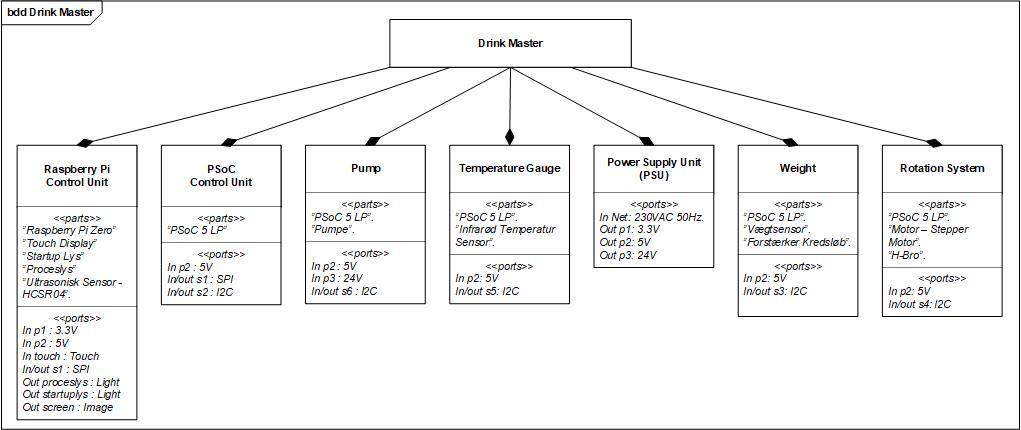
\includegraphics[width=1.2\textwidth, angle =270]{Images/BDD_System_JPEG.jpg}
	\caption{bdd for Drink master}
	\label{fig:bdd}
\end{figure}
\FloatBarrier

\begin{table}[H] 
	\centering 
	\caption{Blokbeskrivelse for figur \ref{fig:bdd} bdd Drink master}
	\begin{tabular}{|p{3cm}|p{7cm}|p{3cm}|}
		\hline
\textbf{Bloknavn} & \textbf{Funktionsbeskrivelse}  &  \textbf{Kommentar}  \\ \hline
Raspberry Pi control unit    & Raspberry Pi SPI Master-enhed. Er forbundet med et Touch Display, som er brugerens tilgang til systemet. Der er også forbundet med en ultralydssensor som tænder lys i system når en bruger er tæt på. Kommunikerer med PSoC I2C Master-enhed. &  \\ \hline
PSoC control unit & I2C Master-enhed, som kommunikerer direkte med alle andre enheder. Danner et kommunikationsled mellem alle I2C PSoC Slaver og RPi SPI Master.    &  \\ \hline
Pump              & En pumpe der pumper en prædefineret mængde af væske fra en flaske ned i et indsat krus, som skal mixes i den valgte drink.                       &  \\ \hline
Temperature Gauge & En Infrarød Temperatur Sensor detekterer temperaturen på flasker.                                                                                &  \\ \hline
PSU               & En strømforsyning som leverer de forskellige spændinger som systemet har brug for.                                                                               &  \\  \hline
Weight            & Et vægtsystem til at registrere indsat krus, før en drik kan laves, og om væske er påfyldt kruset.                                                                      &  \\ \hline
Rotation System   & En motor styrer et hjul med flasker. En flaske, som skal bruges til en valgt drink bliver positioneret ovenover et indsat krus.                  &  \\ \hline

		\hline 
	\end{tabular}
	\label{tab:blokbeskrivelse}
\end{table}
\FloatBarrier

\begin{figure}[h!]
	\centering
	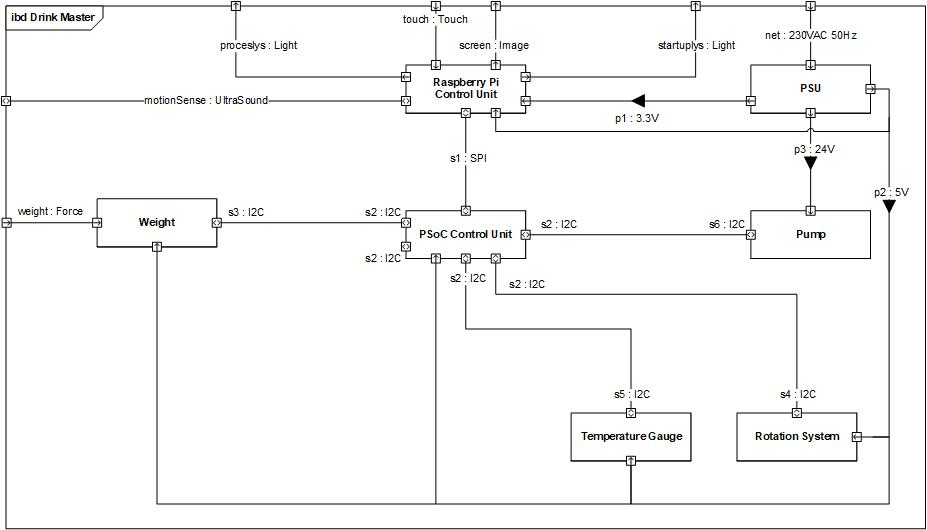
\includegraphics[width=1\textwidth]{Images/IBD_System_JPEG.jpg}
	\caption{ibd for Drink master}
	\label{fig:ibd}
\end{figure}
\FloatBarrier

\begin{table}[H] 
	\centering 
	\caption{Signalbeskrivelse for figur \ref{fig:ibd} ibd Drink master}
	\begin{tabular}{|p{3cm}|p{7cm}|p{3cm}|}
		\hline
\textbf{Signal} & \textbf{Funktionsbeskrivelse}  &  \textbf{Kommentar}  \\ \hline
Raspberry Pi control unit   & &  \\ \hline
PSoC control unit    & &  \\ \hline
Pump              & &  \\ \hline
Temperature Gauge & &  \\ \hline
PSU               & &  \\ \hline 
Weight            & &  \\ \hline
Rotation System   & &  \\ \hline

	\end{tabular}
	\label{tab:signalbeskrivelse}
\end{table}
\FloatBarrier
%\title{Test use cases og navneord\\
\chapter{Systemarkitektur - Software}
\section{Navneord fra use case}

\begin{itemize}
    \item RPi
    \item GUI
    \item Master PSoC
    \item Slave PSoC
\end{itemize}

\section{Use cases}
\subsection{UC1: Bestil drink}
\begin{table}[H]
\begin{tabular}{|p{5cm}|p{9cm}|}
\hline
\rowcolor[HTML]{C0C0C0} 
\textbf{Navn:} & Bestil drink\\ \hline
\textbf{Mål:} & Bruger modtager den bestilte drink\\ \hline
\rowcolor[HTML]{C0C0C0} 
\textbf{Initiering:} & Bruger går over til touchskærmen som tænder\\ \hline
\textbf{Aktører:} & Bruger/ejer\\ \hline
\rowcolor[HTML]{C0C0C0} 
\textbf{Antal samtidige forekomster:} & ingen\\ \hline
\textbf{Prækondition:} & Drinkmaster er funktionsdygtig og brugeren har placeret et glas i systemet. \\ \hline
\rowcolor[HTML]{C0C0C0} 
\textbf{Postkondition:} & Kunden tager den bestilte drink\\ \hline
\begin{tabular}[c]{@{}l@{}} \textbf{Hovedscenarie:} \\ \\ \\ \\ \\ \\ \\ \\ \\ \\ \end{tabular}& \begin{tabular}[c]{@{}l@{}}
1. Systemets touchscreen viser en liste af mulige drinks.\\
2. Brugeren vælger drink på touchscreen.\\
3. Systemet modtager brugerens valg.\\
4. Systemet undersøger om der er tilstrækkelige mængder \\ \hspace*{4mm}af ingredienser til at lave drinken. \\\hspace*{4mm}\textit{[EXT 1: Ikke tilstrækkelige mængder af ingredienser]}\\
5. Systemet doserer drinkens ingredienser i glasset. \\
6. Systemet viser beskeden ”Valgte drink er klar – tag \\ \hspace*{4mm}din drink” på touchscreen.\\
7. Brugeren tager glasset med drinken og UC afsluttes. \\
\end{tabular}\\ \hline
\rowcolor[HTML]{C0C0C0} 
\textbf{Udvidelser/undtagelser:} & \begin{tabular}[c]{@{}l@{}}
\textit{[EXT 1: Ikke tilstrækkelige mængder af ingredienser]}\\ 
1. UC 4 initieres.\\
2. UC 4 afsluttes og use casen returnerer til punkt 5. \\
\end{tabular}\\ \hline
\end{tabular}
\end{table}

\subsection{UC2: Lav egen drink}
\begin{table}[H]
\begin{tabular}{|p{5cm}|p{9cm}|}
\hline
\rowcolor[HTML]{C0C0C0} 
\textbf{Navn:} & Lave egen drink\\ \hline
\textbf{Mål:} & At brugeren tilføjer en drink til databasen\\ \hline
\rowcolor[HTML]{C0C0C0} 
\textbf{Initiering:} & Bruger går over til drink master maskinen.\\ \hline
\textbf{Aktører:} & Bruger/ejer\\ \hline
\rowcolor[HTML]{C0C0C0} 
\textbf{Antal samtidige forekomster:} & ingen\\ \hline
\textbf{Prækondition:} & Maskinen er tændt og aktiveret\\ \hline
\rowcolor[HTML]{C0C0C0} 
\textbf{Postkondition:} & Der er oprettet en brugerdefineret drink i databasen og maskinen er klar til næste operation\\ \hline
\begin{tabular}[c]{@{}l@{}} \textbf{Hovedscenarie:} \\ \\ \\ \\ \\ \\ \\ \\ \\\end{tabular}& \begin{tabular}[c]{@{}l@{}}
1. Systemet registrerer bruger er indenfor rækkevidde og \\\hspace*{4mm}touchskærm tænder. \\
2. Bruger vælger “Lav egen drink”. \\
3. Bruger bedes indtaste et navn på den ønskede drink. \\
4. Bruger indtaster navn på drink og trykker “Ok” \\
5. En liste over tilgængelig alkohol/mixere vises. \\
6. Bruger vælger de ønskede væsker, og mængde. \\
7. Bruger trykker tilføj drink \\
\hspace*{4mm}\textit{[EXT 1]: Bruger trykker annullér} \\

\end{tabular}\\ \hline
\rowcolor[HTML]{C0C0C0} 
\textbf{Udvidelser/undtagelser:} & \textit{[EXT 1] Bruger trykker annullér}
\item 1. Bruger returneres til startskærmen.
\item 2. De valgt indstillinger slettes\\ \hline
\end{tabular}
\end{table}

\subsection{UC3: Slet drink}
\begin{table}[H]
\begin{tabular}{|p{5cm}|p{9cm}|}
\hline
\rowcolor[HTML]{C0C0C0} 
\textbf{Navn:} & Slet drink\\ \hline
\textbf{Mål:} & At ejeren har slettet en drink i listen over drinks\\ \hline
\rowcolor[HTML]{C0C0C0} 
\textbf{Initiering:} & Ejer vælger slet drik.\\ \hline
\textbf{Aktører:} & Ejer\\ \hline
\rowcolor[HTML]{C0C0C0} 
\textbf{Antal samtidige forekomster:} & ingen\\ \hline
\textbf{Prækondition:} & Ejer har tilstrækkelige rettigheder til at kunne slette en drink fra databasen. Touchskærmen er tændt.\\ \hline
\rowcolor[HTML]{C0C0C0} 
\textbf{Postkondition:} & En drink er blevet slettet fra drinkdatabasen og dette er også opdateret på listen til maskinen.\\ \hline
\textbf{Hovedscenarie:} & 
1. Ejer vælger "Slet drink" på touchskærmen
\item 2. En liste over nuværende drinks vises til brugeren.
\item 3. Ejeren trykker på den drink som ønskes slettet. 
\item 4. Touchskærmen viser en besked:” Vil du slette den valgte \hspace*{4mm}drink?”
\item 5. Ejer trykker på Ja \newline
\hspace*{4mm}\textit{[Ext 1: Ejer trykker på nej]}
\item 6. Touch skærm udskriver ”Drink slettet”
\item 7. Use case afsluttet
\\ \hline
\rowcolor[HTML]{C0C0C0} 
\textbf{Udvidelser/undtagelser:} & \textit{[EXT 1] Ejeren annullerer sletning af drink}
\item1. Ejer trykker på nej
\item2. Applikationen går tilbage til siden led listen over drinks.
\item3. Use case afsluttes \\ \hline
\end{tabular}
\end{table}

\subsection{UC4: Påfyld ingredienser}
\begin{table}[H]
\begin{tabular}{|p{5cm}|p{9cm}|}
\hline
\rowcolor[HTML]{C0C0C0} 
\textbf{Navn:} & Påfyld ingredienser\\ \hline
\textbf{Mål:} & At fylde ingredienser i maskinen\\ \hline
\rowcolor[HTML]{C0C0C0} 
\textbf{Initiering:} & Ejer går hen til maskinen\\ \hline
\textbf{Aktører:} & Ejer\\ \hline
\rowcolor[HTML]{C0C0C0} 
\textbf{Antal samtidige forekomster:} & ingen\\ \hline
\textbf{Prækondition:} & Indholdet i en af flaskerne er 10 cl. eller under.\\ \hline
\rowcolor[HTML]{C0C0C0} 
\textbf{Postkondition:} & Den valgte ingrediens er tilføjet og maskinen er funktionsdygtig\\ \hline
\begin{tabular}[c]{@{}l@{}} \textbf{Hovedscenarie:} \\ \\ \\ \\ \\ \\ \\ \\\end{tabular}& \begin{tabular}[c]{@{}l@{}}
1. Touchskærmen giver besked om at en eller flere \\\hspace*{4mm}ingredienser skal genopfyldes. \\
2. Ejer vælger “Udskift ingrediens” \\
3. Ejer afmonterer den valgte flaske og påsætter den nye \\\hspace*{4mm}flaske. \\
4. Ejer trykker herefter på touch displayet \\\hspace*{4mm}“Ingrediens udskiftet”. \\
5. Touchskærmen returnerer til hovedmenu \\
6. Use case afsluttes\\
\end{tabular}\\ \hline
\rowcolor[HTML]{C0C0C0} 
\textbf{Udvidelser/undtagelser:} & Ingen
\end{tabular}
\end{table}

\section{Test Use cases:}

\begin{itemize}
    \item Registrer bruger
    \item Vægt registrerer kop
    \item Ændre flaskeposition
    \item Doser væske
    \item Registrer tom flaske
    \item PSoC master fortæller RPi at drink er færdig
\end{itemize}

\subsection{TUC 1: Registrer bruger}
\begin{table}[H]
\begin{tabular}{|p{5cm}|p{9cm}|}
\hline
\rowcolor[HTML]{C0C0C0} 
\textbf{Navn:} & Registrer bruger\\ \hline
\textbf{Mål:} & Motionsensor registrere bruger og tænder for touchscreen\\ \hline
\rowcolor[HTML]{C0C0C0} 
\textbf{Initiering:} & Bruger\\ \hline
\textbf{Aktører:} & Bruger\\ \hline
\rowcolor[HTML]{C0C0C0} 
\textbf{Antal samtidige forekomster:} & 1\\ \hline
\textbf{Prækondition:} & Touchscreen er slukket \\ \hline
\rowcolor[HTML]{C0C0C0} 
\textbf{Postkondition:} & Touchscreen er tændt og systemet er klar til at modtage bestilling.\\ \hline
\begin{tabular}[c]{@{}l@{}} \textbf{Hovedscenarie:} \\ \\ \\ \\\end{tabular}& \begin{tabular}[c]{@{}l@{}}
1. Bruger går hen til systemet. \\
2. Proximitysensor registrerer bruger. \\
\usepackage{}3. Proximitysensor sender signal til RPi. \\
4. RPi tænder for touchscreen. \\
\end{tabular}\\ \hline
\rowcolor[HTML]{C0C0C0} 
\textbf{Udvidelser/undtagelser:} & Ingen\\ \hline
\end{tabular}
\end{table}

\subsection{TUC 2: Vægt registrerer kop}
\begin{table}[H]
\begin{tabular}{|p{5cm}|p{9cm}|}
\hline
\rowcolor[HTML]{C0C0C0} 
\textbf{Navn:} & Vægt registrerer kop\\ \hline
\textbf{Mål:} & Vægt registrere kop og enabler "bestil drink"\\ \hline
\rowcolor[HTML]{C0C0C0} 
\textbf{Initiering:} & Bruger\\ \hline
\textbf{Aktører:} & Bruger\\ \hline
\rowcolor[HTML]{C0C0C0} 
\textbf{Antal samtidige forekomster:} & 1\\ \hline
\textbf{Prækondition:} & Der står ikke en kop i forvejen og systemet er ikke i gang med at brygge en drink.\\ \hline
\rowcolor[HTML]{C0C0C0} 
\textbf{Postkondition:} & \begin{tabular}[c]{@{}l@{}}Knappen "bryg drink" på touchskærm er enabled\end{tabular} \\ \hline
\begin{tabular}[c]{@{}l@{}} \textbf{Hovedscenarie:} \\ \\ \\ \\ \\ \end{tabular} & \begin{tabular}[c]{@{}l@{}}
1. Bruger sætter sin kop til opfylding. \\
2. Vægtens load cell sender signaler til PSoC Slave. \\
4. PSoC Slave sender data til PSoC master. \\
5. PSoC Master sender data til RPi \\
6. RPi enabler "Bryg drink" på GUI \\
\end{tabular}\\ \hline
\rowcolor[HTML]{C0C0C0} 
\textbf{Udvidelser/undtagelser:} & \\ \hline
\end{tabular}
\end{table}

\subsection{TUC 3: Ændre flaskeposition}
\begin{table}[H]
\begin{tabular}{|p{5cm}|p{9cm}|}
\hline
\rowcolor[HTML]{C0C0C0} 
\textbf{Navn:} & Ændre flaskeposition.\\ \hline
\textbf{Mål:} & Systemet drejer ønsket flaske frem til doseringspositionen\\ \hline
\rowcolor[HTML]{C0C0C0} 
\textbf{Initiering:} & Bruger\\ \hline
\textbf{Aktører:} & Bruger\\ \hline
\rowcolor[HTML]{C0C0C0} 
\textbf{Antal samtidige forekomster:} & 1\\ \hline
\textbf{Prækondition:} & Systemet er tændt og klar til brug. \\ \hline
\rowcolor[HTML]{C0C0C0} 
\textbf{Postkondition:} & Systemet har drejet den ønskede flaske frem til doseringspositionen.\\ \hline
\begin{tabular}[c]{@{}l@{}} \textbf{Hovedscenarie:} \\ \\ \\ \\ \\ \\ \\ \end{tabular}& \begin{tabular}[c]{@{}l@{}}
1. Bruger vælger ønsket flaske på touchscreen. \\
2. RPi sender signal til PSoC Master. \\
3. PSoC Master sender signal til PSoC Slave. \\
4. PSoC Slave tænder steppermotor. \\
5. Steppermotor drejer flaskebeholder rundt. \\
6. Steppermotor stopper når ønsket flaske er ved \\doseringsposition. \\
\end{tabular}\\ \hline
\rowcolor[HTML]{C0C0C0} 
\textbf{Udvidelser/undtagelser:} & Ingen\\ \hline
\end{tabular}
\end{table}

\subsection{TUC 4: Doser væske}
\begin{table}[H]
\begin{tabular}{|p{5cm}|p{9cm}|}
\hline
\rowcolor[HTML]{C0C0C0} 
\textbf{Navn:} & Doser væske\\ \hline
\textbf{Mål:} & Systemet doserer den ønskede mængde væske\\ \hline
\rowcolor[HTML]{C0C0C0} 
\textbf{Initiering:} & Bruger\\ \hline
\textbf{Aktører:} & Bruger\\ \hline
\rowcolor[HTML]{C0C0C0} 
\textbf{Antal samtidige forekomster:} & 1\\ \hline
\textbf{Prækondition:} & Systemet er tændt og klar til brug. \\ \hline
\rowcolor[HTML]{C0C0C0} 
\textbf{Postkondition:} & Systemet har doseret den rigtige mængde væske i glasset.\\ \hline
\begin{tabular}[c]{@{}l@{}} \textbf{Hovedscenarie:} \\ \\ \\ \\ \\ \\\end{tabular}& \begin{tabular}[c]{@{}l@{}}
1. Bruger vælger ønsket mængde væske på touchscreen. \\
2. RPi sender besked til PSoC Master. \\
3. PSoC Master sender signal til PSoC Slave. \\
4. PSoC Slave tænder for pumpen ved flasken der er ved\\ doseringspositionen.\\
5. Pumpen stopper når ønsket mængde væske er doseret. \\
\end{tabular}\\ \hline
\rowcolor[HTML]{C0C0C0} 
\textbf{Udvidelser/undtagelser:} & Ingen\\ \hline
\end{tabular}
\end{table}

\subsection{TUC 5: Registrer tom flaske}
\begin{table}[H]
\begin{tabular}{|p{5cm}|p{9cm}|}
\hline
\rowcolor[HTML]{C0C0C0} 
\textbf{Navn:} & Registrer tom flaske \\ \hline
\textbf{Mål:} & Systemet skal registrerer at en flaske indeholder mindre en 10 cl, og sende besked til touchscreen\\ \hline
\rowcolor[HTML]{C0C0C0} 
\textbf{Initiering:} & Bruger går hen til touchskærmen, og motion sensor registrerer bevægelse \\ \hline
\textbf{Aktører:} & Bruger\\ \hline
\rowcolor[HTML]{C0C0C0} 
\textbf{Antal samtidige forekomster:} & 1\\ \hline
\textbf{Prækondition:} & Drinkmaster mangler IKKE service og klar til brug. Den valgte flaske indeholder 70 cl \\ \hline
\rowcolor[HTML]{C0C0C0} 
\textbf{Postkondition:} & Systemet har registreret at en flaskes indhold er 10 cl eller mindre \\ \hline
\begin{tabular}[c]{@{}l@{}} \textbf{Hovedscenarie:} \\ \\ \\ \\\end{tabular}& \begin{tabular}[c]{@{}l@{}}
1. Bruger vælger at doserer 60 cl fra en flaske. \\
2. [Test Use case 4 Initieres med 60 cl] \\
4. Bruger vælger at doserer 5 cl fra samme flaske. \\
5. Rpi udskriver, at flasken er ved at være tom \\
\end{tabular}\\ \hline
\rowcolor[HTML]{C0C0C0} 
\textbf{Udvidelser/undtagelser:} & Ingen\\ \hline
\end{tabular}
\end{table}


\subsection{TUC 6: PSoC master fortæller RPi at drink er færdig}
\begin{table}[H]
\begin{tabular}{|p{5cm}|p{9cm}|}
\hline
\rowcolor[HTML]{C0C0C0} 
\textbf{Navn:} & PSoC master fortæller RPi at drink er færdig\\ \hline
\textbf{Mål:} & RPi har modtaget fra PSoC Master at \\ \hline
\rowcolor[HTML]{C0C0C0} 
\textbf{Initiering:} & PSoC Master\\ \hline
\textbf{Aktører:} & PSoC Master og RPi\\ \hline
\rowcolor[HTML]{C0C0C0} 
\textbf{Antal samtidige forekomster:} & 1\\ \hline
\textbf{Prækondition:} & Brygning af drink er i gang. \\ \hline
\rowcolor[HTML]{C0C0C0} 
\textbf{Postkondition:} & Systemet har doseret den rigtige mængde væske i glasset.\\ \hline
\begin{tabular}[c]{@{}l@{}} \textbf{Hovedscenarie:} \\ \\ \\ \\\end{tabular}& \begin{tabular}[c]{@{}l@{}}
1. PSoC Master registrerer at drink er færdigbrygget. \\
2. PSoC Master sender status til RPi. \\
3. RPi modtager status om at drink er færdig\\
4. RPi udskriver status på touchskærmen\\ 
\end{tabular}\\ \hline
\rowcolor[HTML]{C0C0C0} 
\textbf{Udvidelser/undtagelser:} & Ingen\\ \hline
\end{tabular}
\end{table}

\section{Grænseflader og protokoller}
\subsection{Grænseflader}
RPi'en kører på 3.3 V, hvilket vil sige at PSoC'en også skal gøre dette således at de logiske niveaer stemmer overens. Det samme gælder for PSoC master til PSoC Slave. For kommunikation mellem RPi og PSoC anvendes SPI protokollen. For kommunikation mellem PSoC Master og PSoC Slave anvendes I2C kommunikation.
\subsection{Protokoller}
Vi skal i vore system sende en opskrift, dvs. en lang række instruktioner, mellem forskellige dele i systemet. RPi'en sender den samlede instruktion ved brug af SPI til PSoC Master som så skal uddeligere de forskellige opgaver til de respektive PSoC Slaves ved brug af I2C protokollen. Opskriften består af forskellige instruktioner som fx. at dreje hjulet med flasker et hvist antal grader. Et andet eksempel kunne være at dispensere \textbf{x}ml af flaske nr 2. Ud fa opskriften som findes i drink databasen, udregner RPi'en alle de nødvendige instruktioner som det er nødvendigt at foretage, for at drinken kan laves. Disse sendes herefter i rækkefølge til PSoC Master som så uddelligerer disse opgaver til PSoC Slaves. Herunder kan ses \ref{tab:protokolTabel} med oversættelse af kommandoer:
\begin{table}[H]
\begin{tabular}{|l|l|}
\hline
Instruktion                              & Oversættelse til protokol \\ \hline
Start transmission                       & 1                         \\ \hline
Afslut transmission                      & 0                         \\ \hline
Rotér x grader mod uret                  & rbx                       \\ \hline
Rotér x grader med uret                  & rfx                       \\ \hline
Dispensér x ml af flaske y               & dyx                       \\ \hline
Undersøg om alle instruktioner er udført & ?                         \\ \hline
Prefix efter hver instruktion            & e                         \\ \hline
PSoC Master til RPi - Drink færdig       & y                         \\ \hline
\end{tabular}
\caption{Tabel for oversættelse af kommandoer}
\label{tab:protokolTabel}
\end{table}

Et eksempel på en transmission af en opskrift kan ser herunder med en tilhørende beskrivelse kan ses herunder på \ref{tab:transExample1}
\begin{table}[H]
\centering
\resizebox{\textwidth}{!}{%
\begin{tabular}{|l|l|l|l|l|l|l|l|l|l|l|l|l|l|l|l|l|l|l|l|}
\hline
Data & \cellcolor[HTML]{9698ED} 1 & \cellcolor[HTML]{67FD9A} r & \cellcolor[HTML]{67FD9A} b & \cellcolor[HTML]{67FD9A} 45 & \cellcolor[HTML]{67FD9A} e & \cellcolor[HTML]{FCFF2F} d & \cellcolor[HTML]{FCFF2F} 2 & \cellcolor[HTML]{FCFF2F} 10 & \cellcolor[HTML]{FCFF2F} e & \cellcolor[HTML]{38FFF8} r & \cellcolor[HTML]{38FFF8} f & \cellcolor[HTML]{38FFF8} 200 & \cellcolor[HTML]{38FFF8} 100 & \cellcolor[HTML]{38FFF8} e & \cellcolor[HTML]{FFCCC9} d & \cellcolor[HTML]{FFCCC9} 4 & \cellcolor[HTML]{FFCCC9} 4 & \cellcolor[HTML]{FFCCC9} e & \cellcolor[HTML]{C0C0C0} s \\ \hline
Beskrivelse & Start transmission & \multicolumn{4}{l|}{\begin{tabular}[c]{@{}l@{}}Besked om at rotere \\ 45 grader mod uret\end{tabular}} & \multicolumn{4}{l|}{\begin{tabular}[c]{@{}l@{}}Besked om at dispensere \\ 10 ml fra flaske 2\end{tabular}} & \multicolumn{5}{l|}{\begin{tabular}[c]{@{}l@{}}Besked om at rotere \\ 300 grader med uret\end{tabular}} & \multicolumn{4}{l|}{\begin{tabular}[c]{@{}l@{}}Besked om at dispensere \\ 4 ml fra flaske 4\end{tabular}} & Stop transmission \\ \hline
\end{tabular}%
}
\caption{Eksempel på en transmission af data med forklaringer}
\label{tab:transExample1}
\end{table}



\section{Domænemodel}

\begin{figure}[h!]
	\centering
	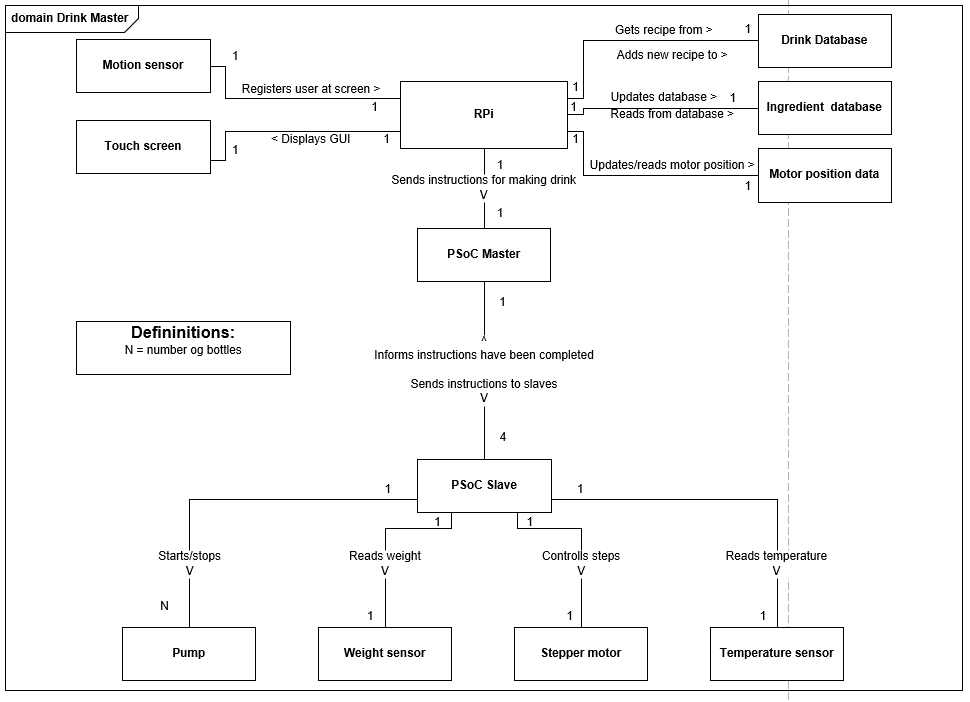
\includegraphics[width=1\textwidth]{Images/domainModel.png}
	\caption{Domæne model for Drink Master}
	\label{fig:domain}
\end{figure}
\section{Acceptestspecifikation af UC}

\subsection{UC 1: Bestil drink}

\begin{table}[H]
\begin{tabular}{|p{1cm}|p{4cm}|p{4cm}|p{4cm}|p{1cm}|}
\hline
\multicolumn{2}{|p{5cm}|}{Use case under test} & \multicolumn{3}{p{9cm}|}{Bestil drink}                                       \\ \hline
\multicolumn{2}{|p{5cm}|}{Scenarie}            & \multicolumn{3}{p{9cm}|}{Hovedscenarie}                                          \\ \hline
\multicolumn{2}{|p{5cm}|}{Prækondition}        & \multicolumn{3}{p{9cm}|}{Drinkmaster er funktionsdygtig og brugeren har placeret etglas i systemet.}                                 \\ \hline
Steps               & Handlinger          & Forventet observation/resultater & Faktisk observation/resultater & OK/ FAIL \\ \hline
1    & Bruger vælger drinken "Vodka/cola" på touchscreen.  & Systemet modtager brugerens valg og undersøger om der er tilstrækkelige mængder af ingredienser til at lave drinken. Systemet doserer 2 cl vodka og 20 cl cola og viser beskeden ”Valgte drink er klar – tag din drink” på touchscreen når drinken er færdig. &   &         \\ \hline
2    & Bruger tager glasset med drinken.  & Systemet returnerer til hovedmenuen. &   &         \\ \hline

\end{tabular}
\end{table}

\subsection{UC 2: Lav egen drink}

\begin{table}[H]
\begin{tabular}{|p{1cm}|p{4cm}|p{4cm}|p{4cm}|p{1cm}|}
\hline
\multicolumn{2}{|p{5cm}|}{Use case under test} & \multicolumn{3}{p{9cm}|}{Lav egen drink}                                       \\ \hline
\multicolumn{2}{|p{5cm}|}{Scenarie}            & \multicolumn{3}{p{9cm}|}{Hovedscenarie}                                          \\ \hline
\multicolumn{2}{|p{5cm}|}{Prækondition}        & \multicolumn{3}{p{9cm}|}{Maskinen er tændt og aktiveret}                                 \\ \hline
Steps               & Handlinger          & Forventet observation/resultater & Faktisk observation/resultater & OK/ FAIL \\ \hline
1    & Bruger vælger "Lav egen drink"  & System anmoder om navn til drinken &   &         \\ \hline
2    & Bruger indtaster "Vodka/juice" og trykker "OK"  & Systemet viser en liste over tilgængelig alkohol og mixere.  &   &         \\ \hline
3    & Bruger vælger 2 cl. vodka og 20 cl. juice "tilføj drink"  & Systemet gemmer drinken i databasen.  &   &         \\ \hline

\end{tabular}
\end{table}

\subsection{UC 3: Slet drink}

\begin{table}[H]
\begin{tabular}{|p{1cm}|p{4cm}|p{4cm}|p{4cm}|p{1cm}|}
\hline
\multicolumn{2}{|p{5cm}|}{Use case under test} & \multicolumn{3}{p{9cm}|}{Slet drink}                                       \\ \hline
\multicolumn{2}{|p{5cm}|}{Scenarie}            & \multicolumn{3}{p{9cm}|}{Hovedscenarie}                                          \\ \hline
\multicolumn{2}{|p{5cm}|}{Prækondition}        & \multicolumn{3}{p{9cm}|}{Ejer har tilstrækkelige rettigheder til at kunne slette en drink fra databasen. Touchskærmen er tændt.}                                 \\ \hline
Steps               & Handlinger          & Forventet observation/resultater & Faktisk observation/resultater & OK/ FAIL \\ \hline
1    & Ejer vælger "Slet drink"på touchskærmen.  & System viser en liste over drinks i databasen. &   &         \\ \hline
2    & Bruger vælger "Vodka/juice" og trykker "OK"  & Systemet viser beskeden ”Vil du slette den valgtedrink?”.  &   &         \\ \hline
3    & Ejer trykker på "Ja".  & Systemet sletter drinken i databasen, og udskriver beskeden "Drink slettet".  &   &         \\ \hline

\end{tabular}
\end{table}

\subsection{UC 4: Påfyld ingredienser}

\begin{table}[H]
\begin{tabular}{|p{1cm}|p{4cm}|p{4cm}|p{4cm}|p{1cm}|}
\hline
\multicolumn{2}{|p{5cm}|}{Use case under test} & \multicolumn{3}{p{9cm}|}{Påfyld ingredienser}                                       \\ \hline
\multicolumn{2}{|p{5cm}|}{Scenarie}            & \multicolumn{3}{p{9cm}|}{Hovedscenarie}                                          \\ \hline
\multicolumn{2}{|p{5cm}|}{Prækondition}        & \multicolumn{3}{p{9cm}|}{Indholdet i vodkaflasken er 10 cl. eller under.}                                 \\ \hline
Steps               & Handlinger          & Forventet observation/resultater & Faktisk observation/resultater & OK/ FAIL \\ \hline
1    & Ejer vælger drinken "Vodka/cola" .  & System giver besked om at vodkaflasken skal genopfyldes.&   &         \\ \hline
2    & Ejer vælger “Udskift ingrediens” og afmonterer vodkaflasken og på sætter en ny,  & Systemet returnerer til hovedmenu.  &   &         \\ \hline

\end{tabular}
\end{table}


\section{Acceptestspecifikation af TUC}

\subsection{TUC 1: Registrer bruger}

\begin{table}[H]
\begin{tabular}{|p{1cm}|p{4cm}|p{4cm}|p{4cm}|p{1cm}|}
\hline
\multicolumn{2}{|p{5cm}|}{Use case under test} & \multicolumn{3}{p{9cm}|}{Registrer bruger}                                       \\ \hline
\multicolumn{2}{|p{5cm}|}{Scenarie}            & \multicolumn{3}{p{9cm}|}{Hovedscenarie}                                          \\ \hline
\multicolumn{2}{|p{5cm}|}{Prækondition}        & \multicolumn{3}{p{9cm}|}{Touchscreen er slukket}                                 \\ \hline
Steps               & Handlinger          & Forventet observation/resultater & Faktisk observation/resultater & OK/ FAIL \\ \hline
1    & Bruger går hen til systemet  & Proximitysensor registrerer bruger og sender et signal til RPi, som tænder for touchscreen.  &   &         \\ \hline

\end{tabular}
\end{table}

\subsection{TUC 2: Vægt registrerer kop}

\begin{table}[H]
\begin{tabular}{|p{1cm}|p{4cm}|p{4cm}|p{4cm}|p{1cm}|}
\hline
\multicolumn{2}{|p{5cm}|}{Use case under test} & \multicolumn{3}{p{9cm}|}{Vægt registrerer kop}                                       \\ \hline
\multicolumn{2}{|p{5cm}|}{Scenarie}            & \multicolumn{3}{p{9cm}|}{Hovedscenarie}                                          \\ \hline
\multicolumn{2}{|p{5cm}|}{Prækondition}        & \multicolumn{3}{p{9cm}|}{Der står ikke en kop i forvejen og systemet er ikke i gangmed at brygge en drink.}                                 \\ \hline
Steps               & Handlinger          & Forventet observation/resultater & Faktisk observation/resultater & OK/ FAIL \\ \hline
1    & Bruger sætter sin kop til opfyldning.  &  Vægtens load cell sender signaler til PSoC Slave. PSoC Slave sender data til PSoC Master. PSoC sender data til RPi. RPi enabler "Bryg drink" på GUI. &   &         \\ \hline

\end{tabular}
\end{table}

\subsection{TUC 3: Ændre flaskeposition}

\begin{table}[H]
\begin{tabular}{|p{1cm}|p{4cm}|p{4cm}|p{4cm}|p{1cm}|}
\hline
\multicolumn{2}{|p{5cm}|}{Use case under test} & \multicolumn{3}{p{9cm}|}{Ændre flaskeposition}                                       \\ \hline
\multicolumn{2}{|p{5cm}|}{Scenarie}            & \multicolumn{3}{p{9cm}|}{Hovedscenarie}                                          \\ \hline
\multicolumn{2}{|p{5cm}|}{Prækondition}        & \multicolumn{3}{p{9cm}|}{Systemet er tændt og klar til brug.}                                 \\ \hline
Steps               & Handlinger          & Forventet observation/resultater & Faktisk observation/resultater & OK/ FAIL \\ \hline
1    & Bruger vælger ønsket flaske på touchscreen  &  RPi sender data til PSoC Master. PSoC Master sender data til PSoC Slave som tænder for steppermotoren. Steppermotoren drejer flaskebeholder rundt og stopper når ønsket flaske er ved doseringspositionen. &   &         \\ \hline

\end{tabular}
\end{table}

\subsection{TUC 4: Doser væske}

\begin{table}[H]
\begin{tabular}{|p{1cm}|p{4cm}|p{4cm}|p{4cm}|p{1cm}|}
\hline
\multicolumn{2}{|p{5cm}|}{Use case under test} & \multicolumn{3}{p{9cm}|}{Doser væske}                                       \\ \hline
\multicolumn{2}{|p{5cm}|}{Scenarie}            & \multicolumn{3}{p{9cm}|}{Hovedscenarie}                                          \\ \hline
\multicolumn{2}{|p{5cm}|}{Prækondition}        & \multicolumn{3}{p{9cm}|}{Systemet er tændt og klar til brug.}                                 \\ \hline
Steps               & Handlinger          & Forventet observation/resultater & Faktisk observation/resultater & OK/ FAIL \\ \hline
1    & Bruger vælger ønsket mængde væske på touchscreen.  &  RPi sender besked til PSoC Master som sender signal til PSoC Slave. PSoC Slave tænder for pumpen ved flasken der er ved doseringspositionen. Pumpen stopper når ønsket mængde væske er doseret. &   &         \\ \hline

\end{tabular}
\end{table}

\subsection{TUC 5: Registrer tom flaske}

\begin{table}[H]
\begin{tabular}{|p{1cm}|p{4cm}|p{4cm}|p{4cm}|p{1cm}|}
\hline
\multicolumn{2}{|p{5cm}|}{Use case under test} & \multicolumn{3}{p{9cm}|}{Registrer tom flaske}                                       \\ \hline
\multicolumn{2}{|p{5cm}|}{Scenarie}            & \multicolumn{3}{p{9cm}|}{Hovedscenarie}                                          \\ \hline
\multicolumn{2}{|p{5cm}|}{Prækondition}        & \multicolumn{3}{p{9cm}|}{Drinkmaster mangler IKKE service og klar til brug. Denvalgte flaske indeholder 70 cl.}                                 \\ \hline
Steps               & Handlinger          & Forventet observation/resultater & Faktisk observation/resultater & OK/ FAIL \\ \hline
1    & Bruger vælger at doserer 60 cl fra en flaske.  &  \textit{(TUC 4 initieres med 60 cl.)} &   &         \\ \hline
2   & Bruger vælger at doserer 5 cl fra samme flaske. & RPi udskriver på touchscreen, at flasken er ved at være tom &    &   \\ \hline

\end{tabular}
\end{table}

\subsection{TUC 6: PSoC master fortæller RPi at drink er færdig.}

\begin{table}[H]
\begin{tabular}{|p{1cm}|p{4cm}|p{4cm}|p{4cm}|p{1cm}|}
\hline
\multicolumn{2}{|p{5cm}|}{Use case under test} & \multicolumn{3}{p{9cm}|}{PSoC master fortæller RPi at drink er færdig}                                       \\ \hline
\multicolumn{2}{|p{5cm}|}{Scenarie}            & \multicolumn{3}{p{9cm}|}{Hovedscenarie}                                          \\ \hline
\multicolumn{2}{|p{5cm}|}{Prækondition}        & \multicolumn{3}{p{9cm}|}{Brygning af drink er i gang.}                                 \\ \hline
Steps               & Handlinger          & Forventet observation/resultater & Faktisk observation/resultater & OK/ FAIL \\ \hline
1    & Ingen  &   Drinken brygges. PSoC Master registrerer at drink er færdigbrygget og sender status til RPi. &   &         \\ \hline

\end{tabular}
\end{table}
\section{Sekvensdiagrammer}

\subsection{Navneord fra use case}

For at starte på udarbejdelse af sekvensdiagrammer, er der ud fra UC'es blevet fundet de nedensåtende navneord. Disse er med til at danne grundlag for de \textit{parts} som skal være en del af sekvensdiagrammerne.

\begin{itemize}
    \item RPi
    \item Touchskærm
    \item Master PSoC
    \item Slave PSoC
\end{itemize}

\subsection{Sekvensdiagrammer til UC's}

%Use case 2
\begin{figure}[H]
	\centering
	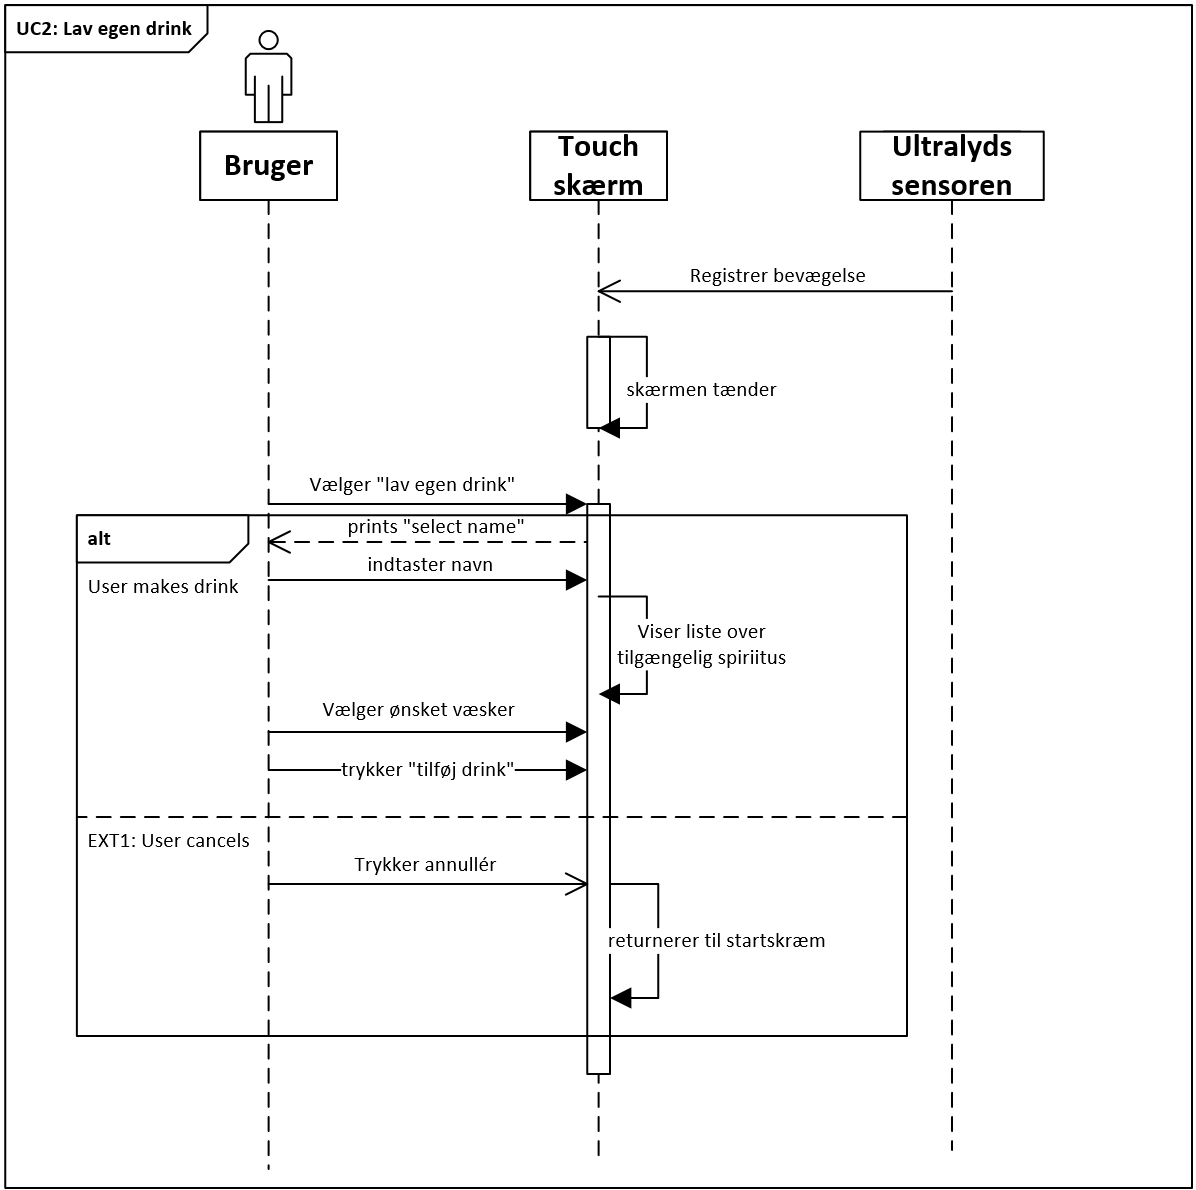
\includegraphics[width=1\textwidth]{Images/UC2lavegendrink.png}
	\caption{Sekvensdiagram for UC2: Lav egen drink }
	\label{fig:UC2}
\end{figure}

%Use case 3
\begin{figure}[H]
	\centering
	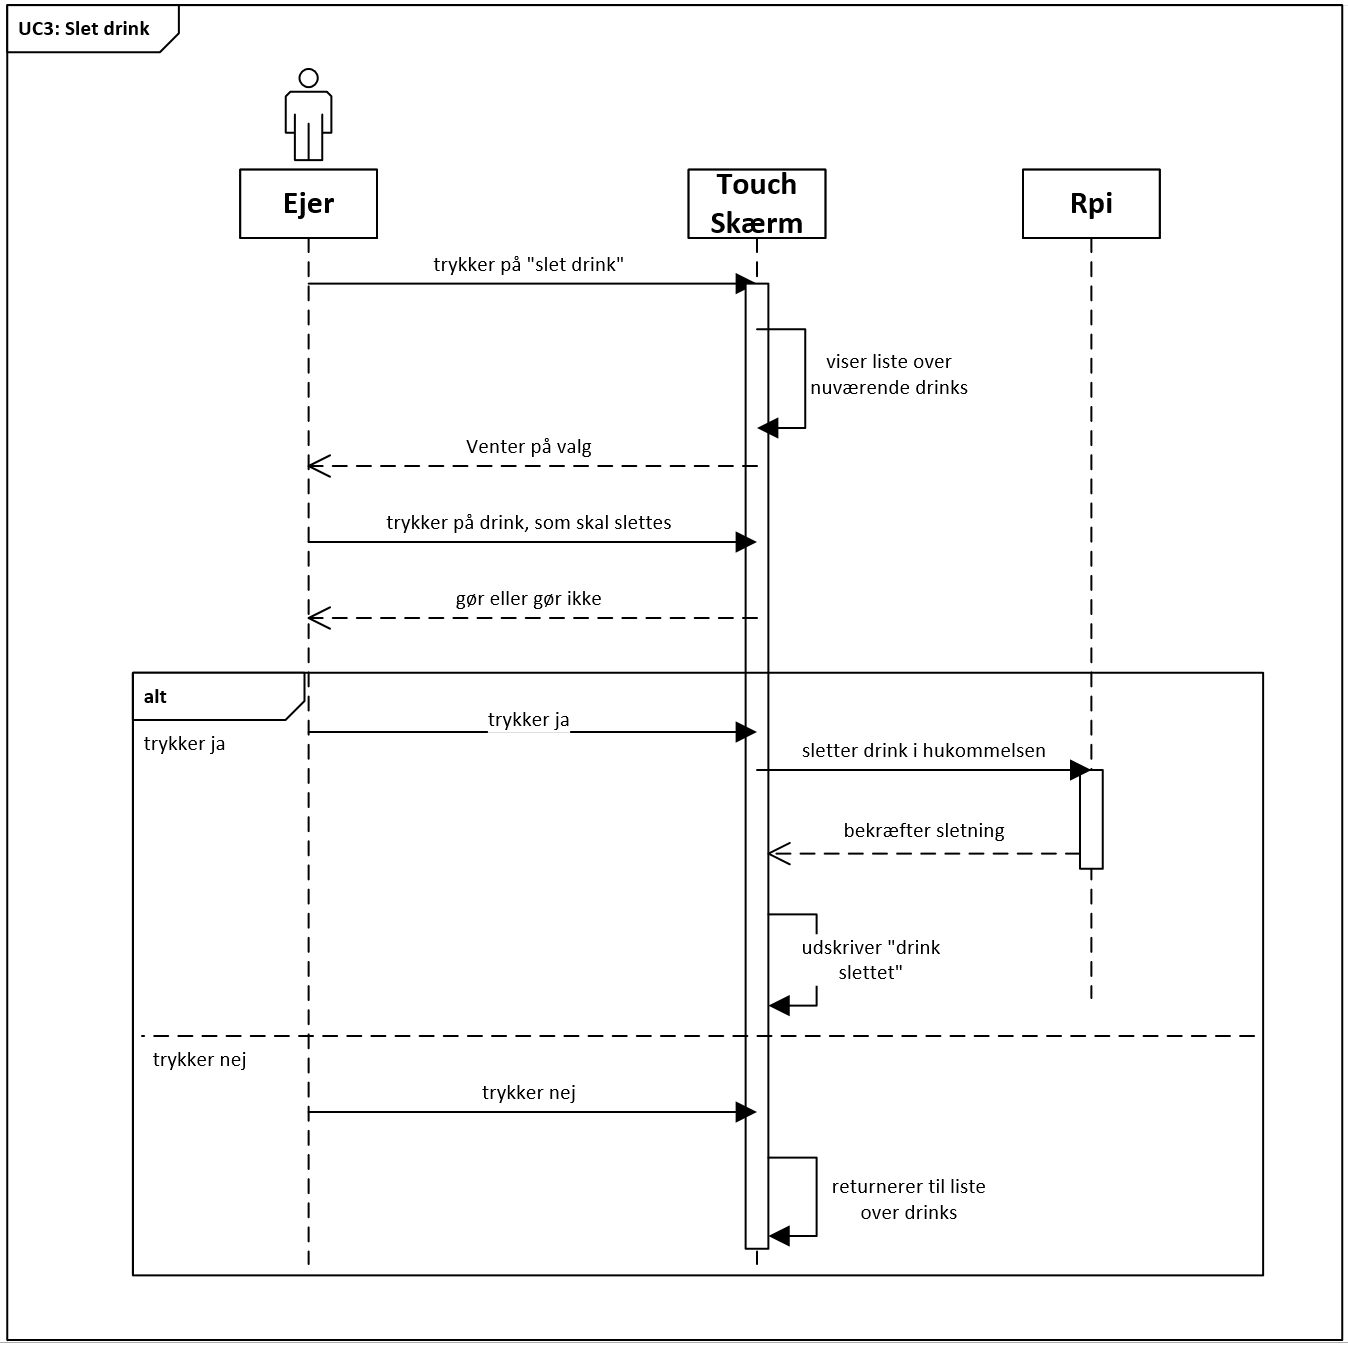
\includegraphics[width=1\textwidth]{Images/UC3sletdrink.png}
	\caption{Sekvensdiagram for UC3: Slet Drink}
	\label{fig:UC3}
\end{figure}

%Use case 4
\begin{figure}[H]
	\centering
	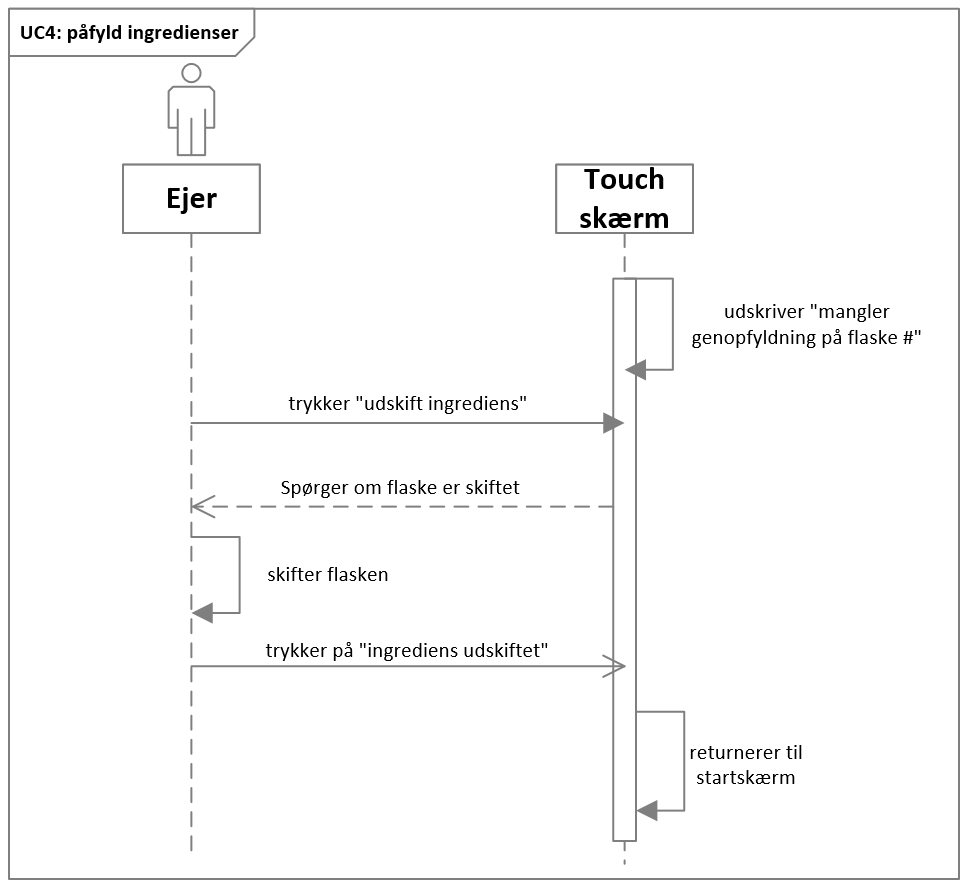
\includegraphics[width=1\textwidth]{Images/UC4paafyldingredienser.png}
	\caption{Sekvensdiagram for UC4: Påfyld ingredienser}
	\label{fig:UC4}
\end{figure}

%Use case 5
\begin{figure}[H]
	\centering
	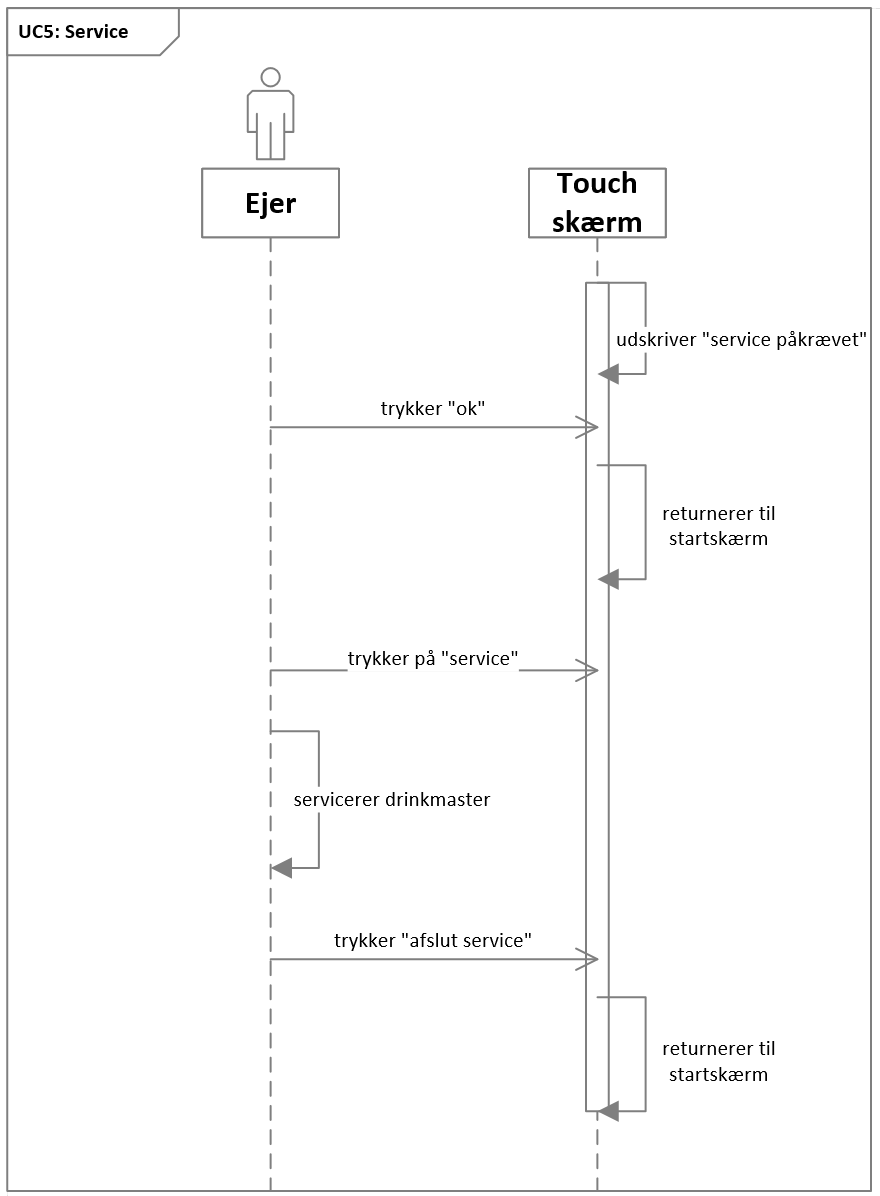
\includegraphics[width=1\textwidth]{Images/UC5service.png}
	\caption{Sekvensdiagram for UC5: Service}
	\label{fig:UC2_service}
\end{figure}

\subsection{Sekvensdiagrammer til test TUC'es}
%Test use case sekvensdiagrammer

\begin{figure}[H]
	\centering
	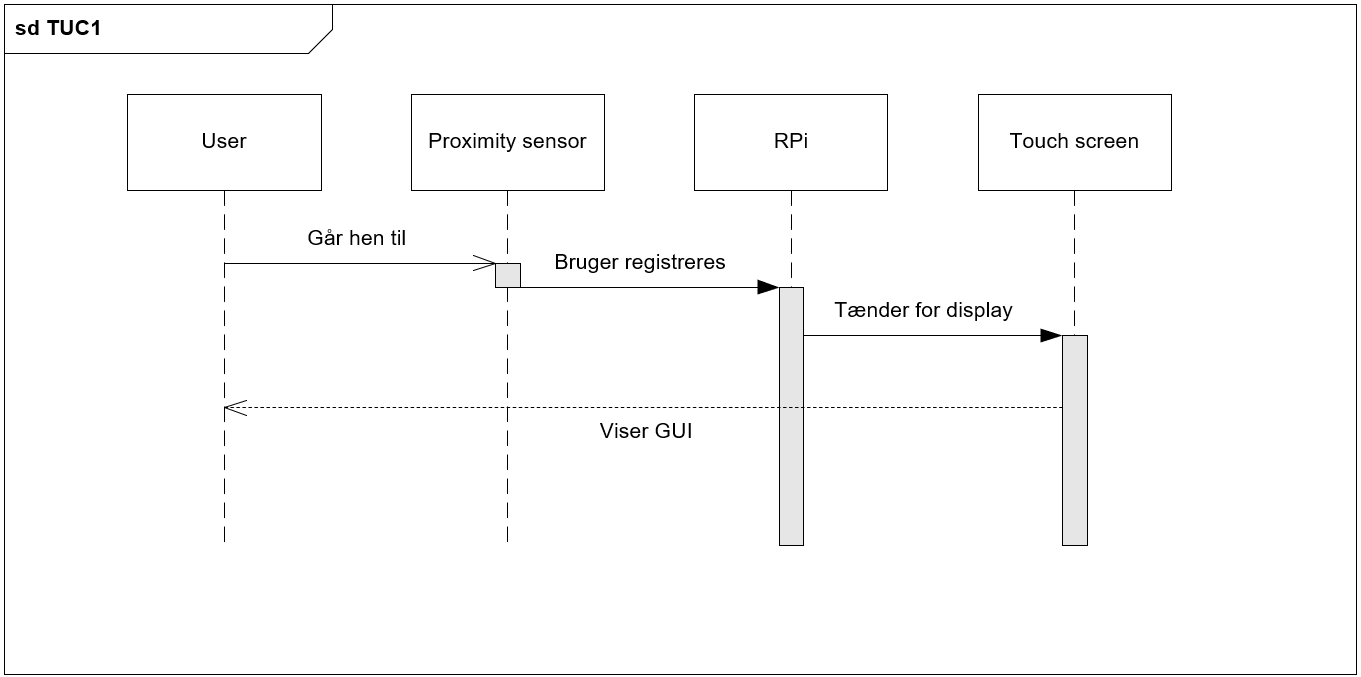
\includegraphics[width=1\textwidth]{Images/TUC1.png}
	\caption{Sekvensdiagram for test TUC1: Registrer bruger}
	\label{fig:testUC1}
\end{figure}

\begin{figure}[H]
	\centering
	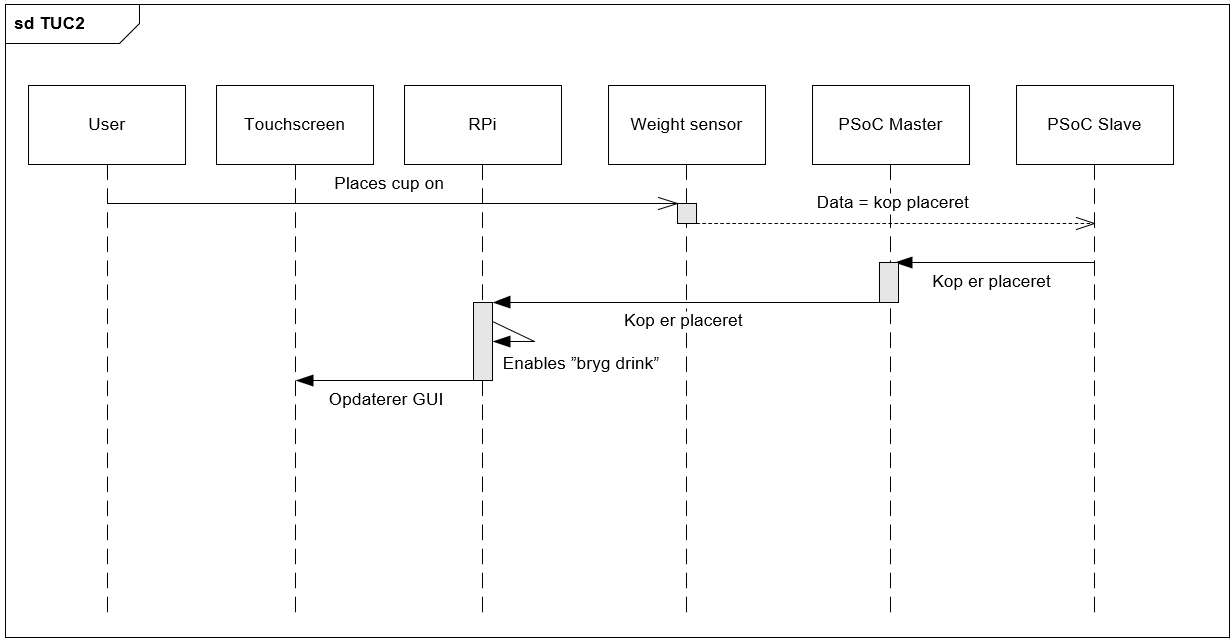
\includegraphics[width=1\textwidth]{Images/TUC2.png}
	\caption{Sekvensdiagram for test TUC2: Vægt registrerer kop}
	\label{fig:testUC2}
\end{figure}

\begin{figure}[H]
	\centering
	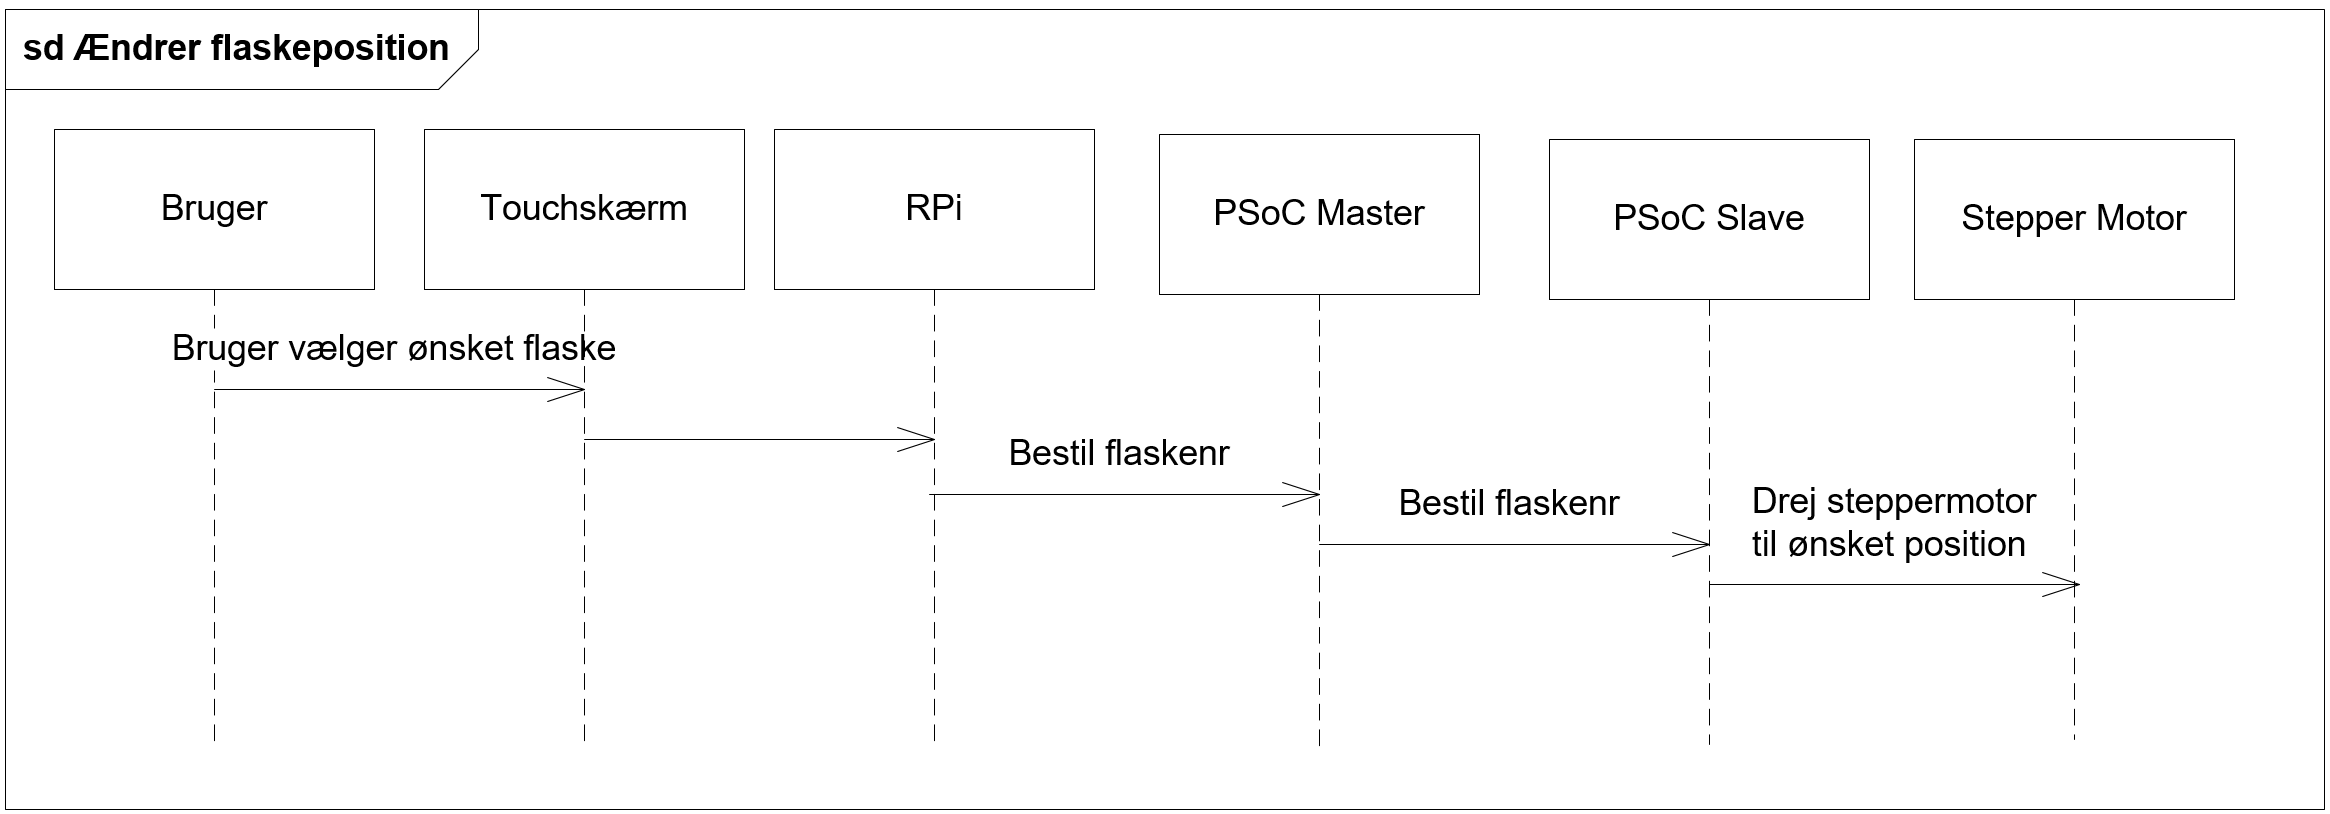
\includegraphics[width=1\textwidth]{Images/sdTestUC3.png}
	\caption{Sekvensdiagram for test TUC3: Ændrer flaskeposition}
	\label{fig:testUC3}
\end{figure}

\begin{figure}[H]
	\centering
	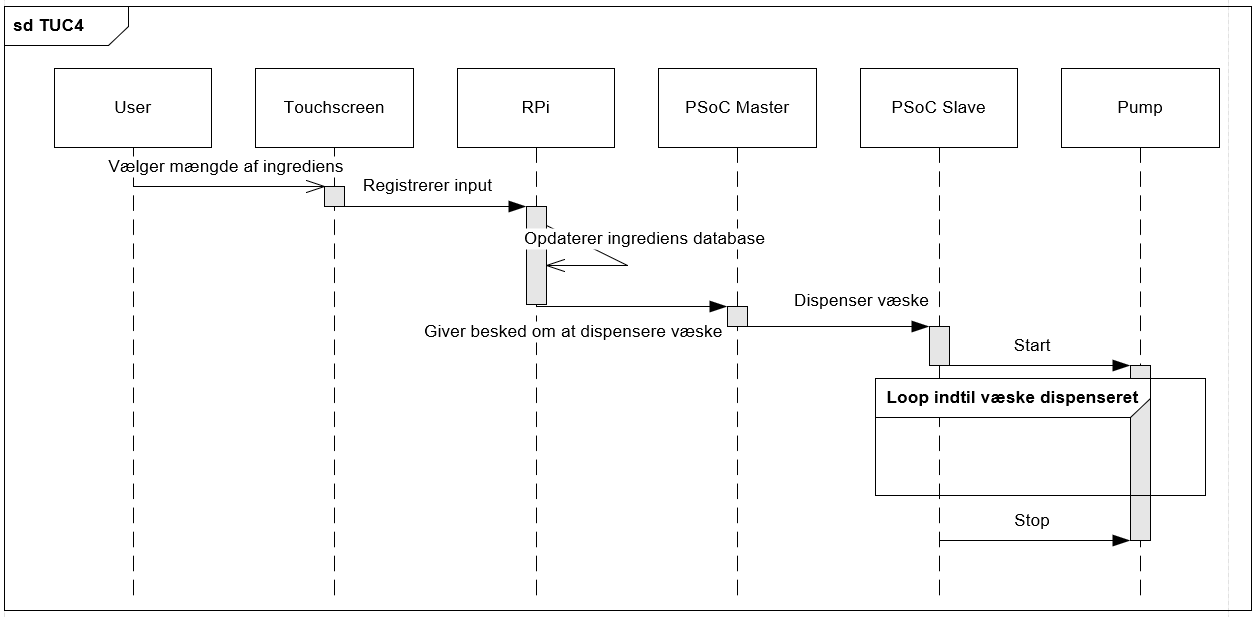
\includegraphics[width=1\textwidth]{Images/TUC4.png}
	\caption{Sekvensdiagram for test TUC4: Doser væske}
	\label{fig:testUC4}
\end{figure}
\begin{figure}[H]
	\centering
	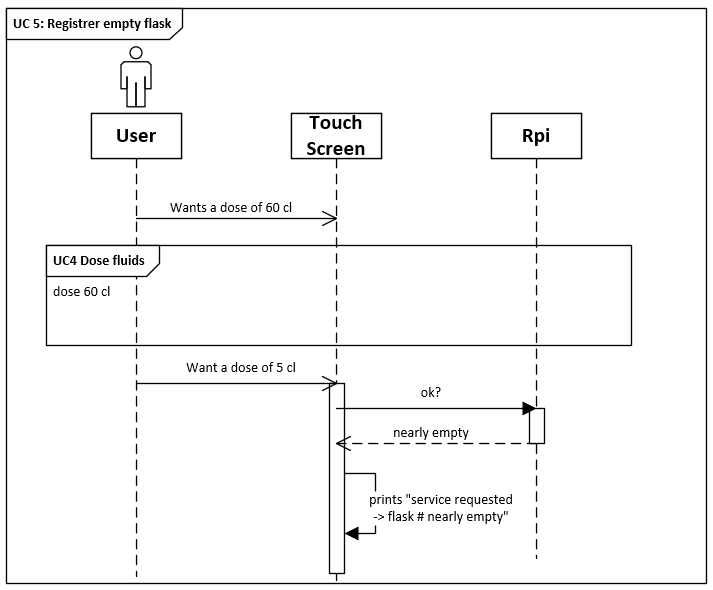
\includegraphics[width=1\textwidth]{Images/testUC5.png}
	\caption{Sekvensdiagram for test TUC5: Registrer tom flaske}
	\label{fig:testUC5}
\end{figure}

\begin{figure}[H]
    \centering
    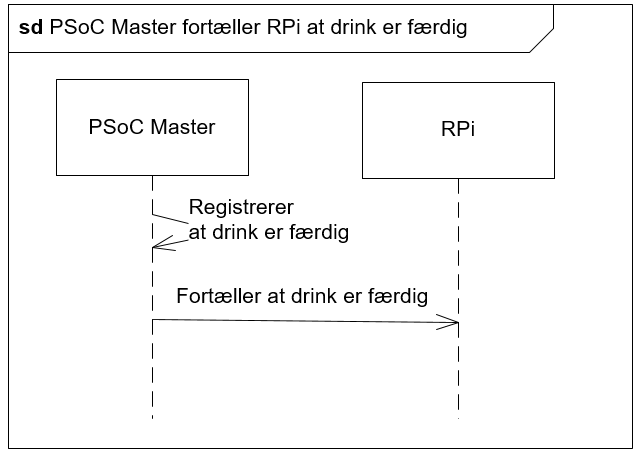
\includegraphics[width=1\textwidth]{Images/sdTestUC6.png}
    \caption{Sekvensdiagram for TUC6: PSoC Master fortæller RPi at drink er færdig}
    \label{fig:testUC6}
\end{figure}
\chapter{Systemarkitektur - software}
\section{Domænemodel}

\begin{figure}[H]
	\centering
	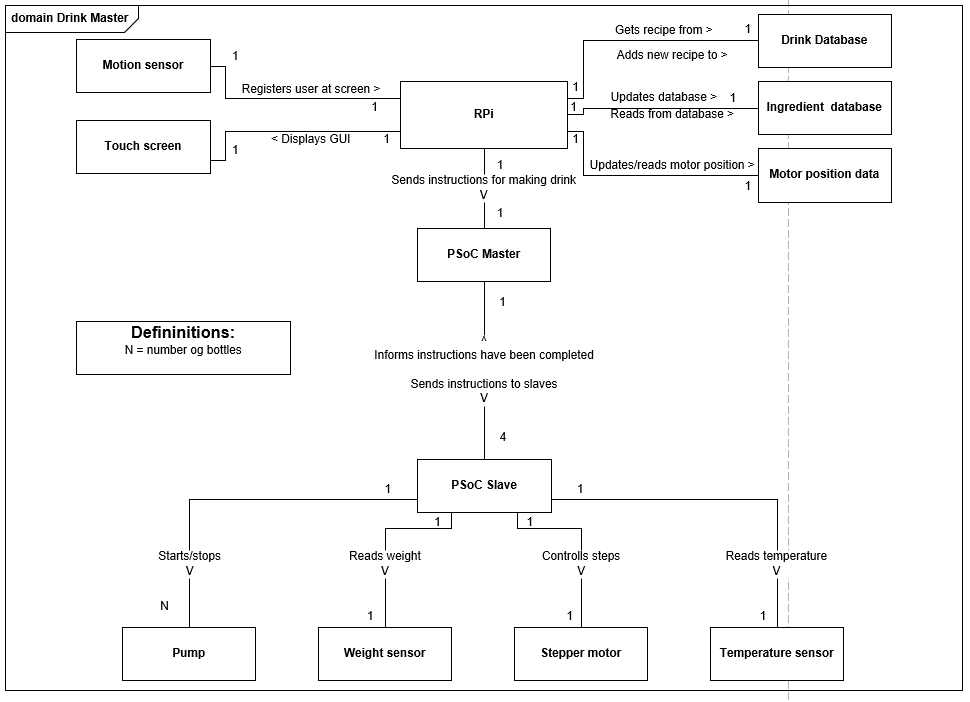
\includegraphics[width=1\textwidth]{Images/domainModel.png}
	\caption{Domæne model for Drink Master}
	\label{fig:domain}
\end{figure}
\section{Sekvensdiagrammer}

\subsection{Navneord fra use case}

For at starte på udarbejdelse af sekvensdiagrammer, er der ud fra UC'es blevet fundet de nedensåtende navneord. Disse er med til at danne grundlag for de \textit{parts} som skal være en del af sekvensdiagrammerne.

\begin{itemize}
    \item RPi
    \item Touchskærm
    \item Master PSoC
    \item Slave PSoC
\end{itemize}

\subsection{Sekvensdiagrammer til UC's}

%Use case 2
\begin{figure}[H]
	\centering
	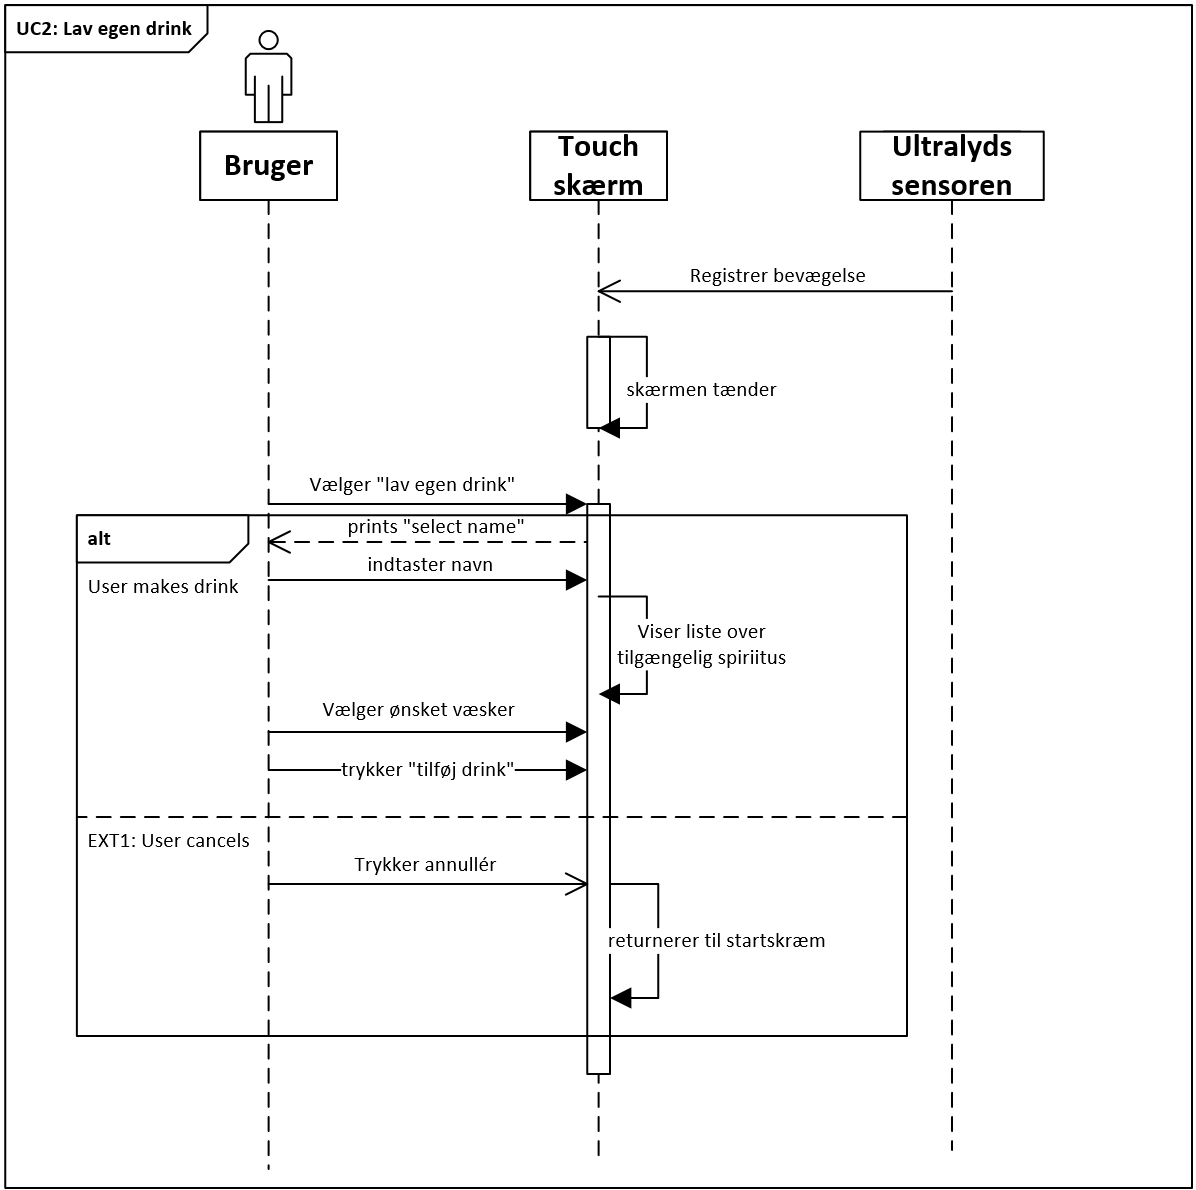
\includegraphics[width=1\textwidth]{Images/UC2lavegendrink.png}
	\caption{Sekvensdiagram for UC2: Lav egen drink }
	\label{fig:UC2}
\end{figure}

%Use case 3
\begin{figure}[H]
	\centering
	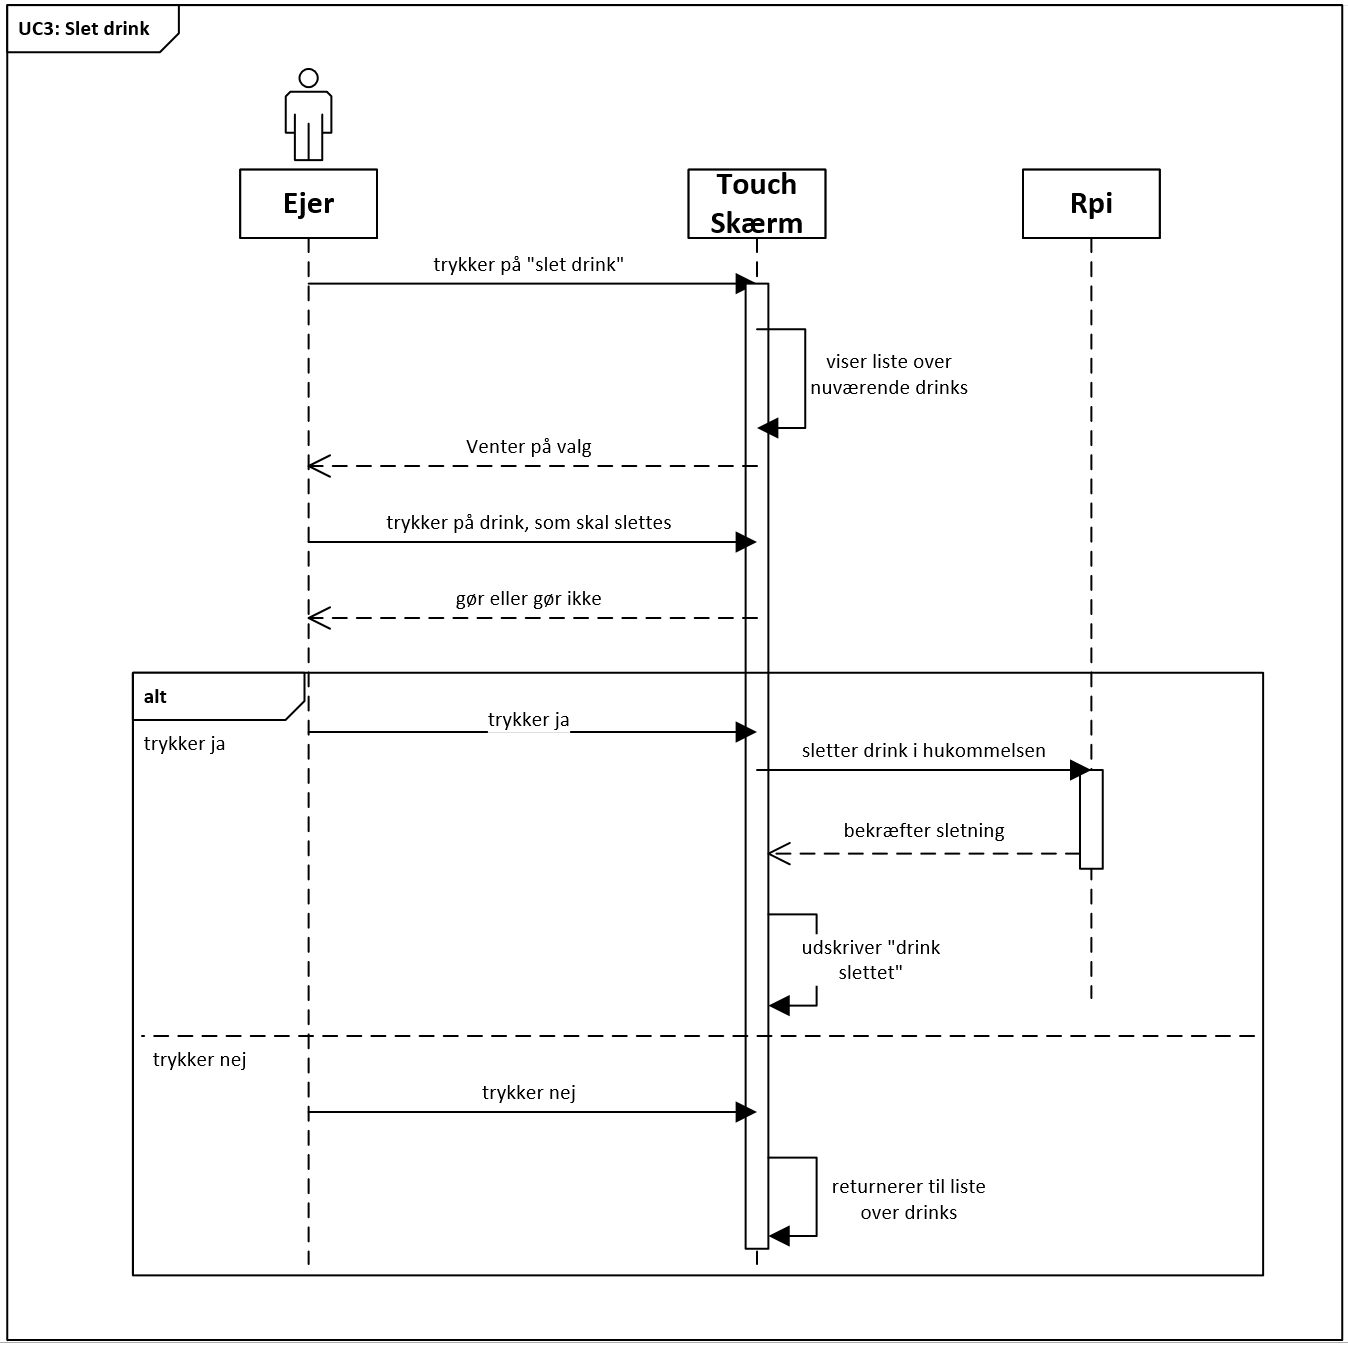
\includegraphics[width=1\textwidth]{Images/UC3sletdrink.png}
	\caption{Sekvensdiagram for UC3: Slet Drink}
	\label{fig:UC3}
\end{figure}

%Use case 4
\begin{figure}[H]
	\centering
	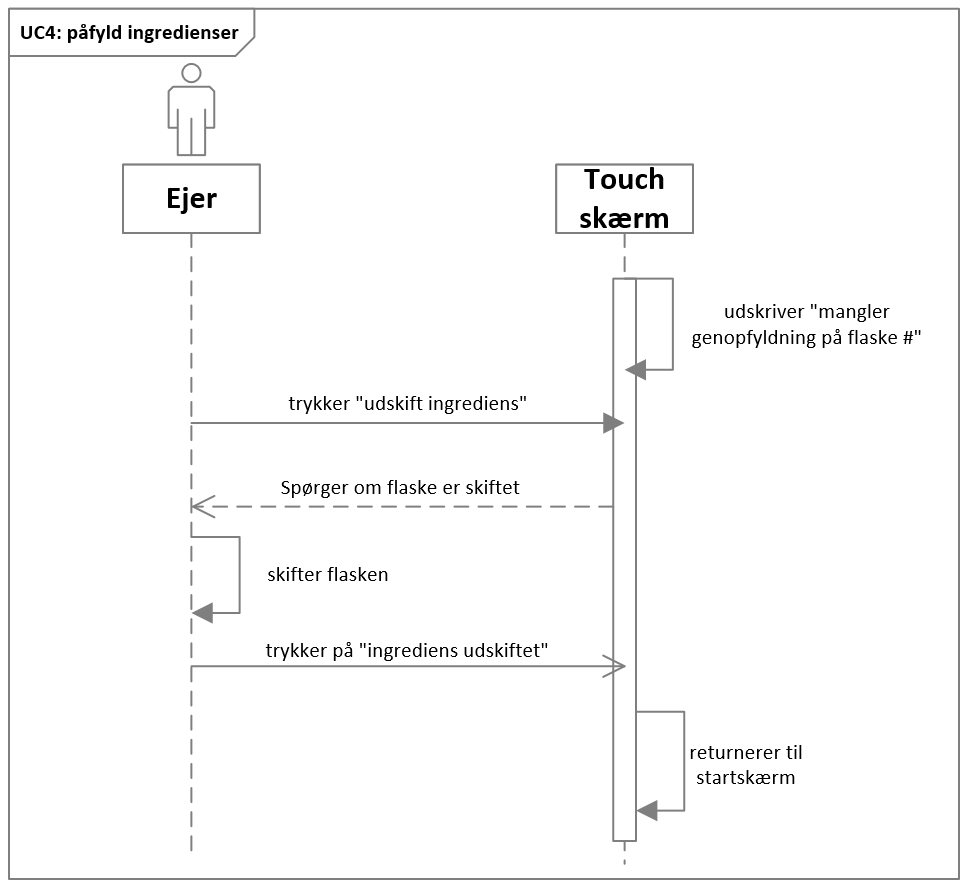
\includegraphics[width=1\textwidth]{Images/UC4paafyldingredienser.png}
	\caption{Sekvensdiagram for UC4: Påfyld ingredienser}
	\label{fig:UC4}
\end{figure}

%Use case 5
\begin{figure}[H]
	\centering
	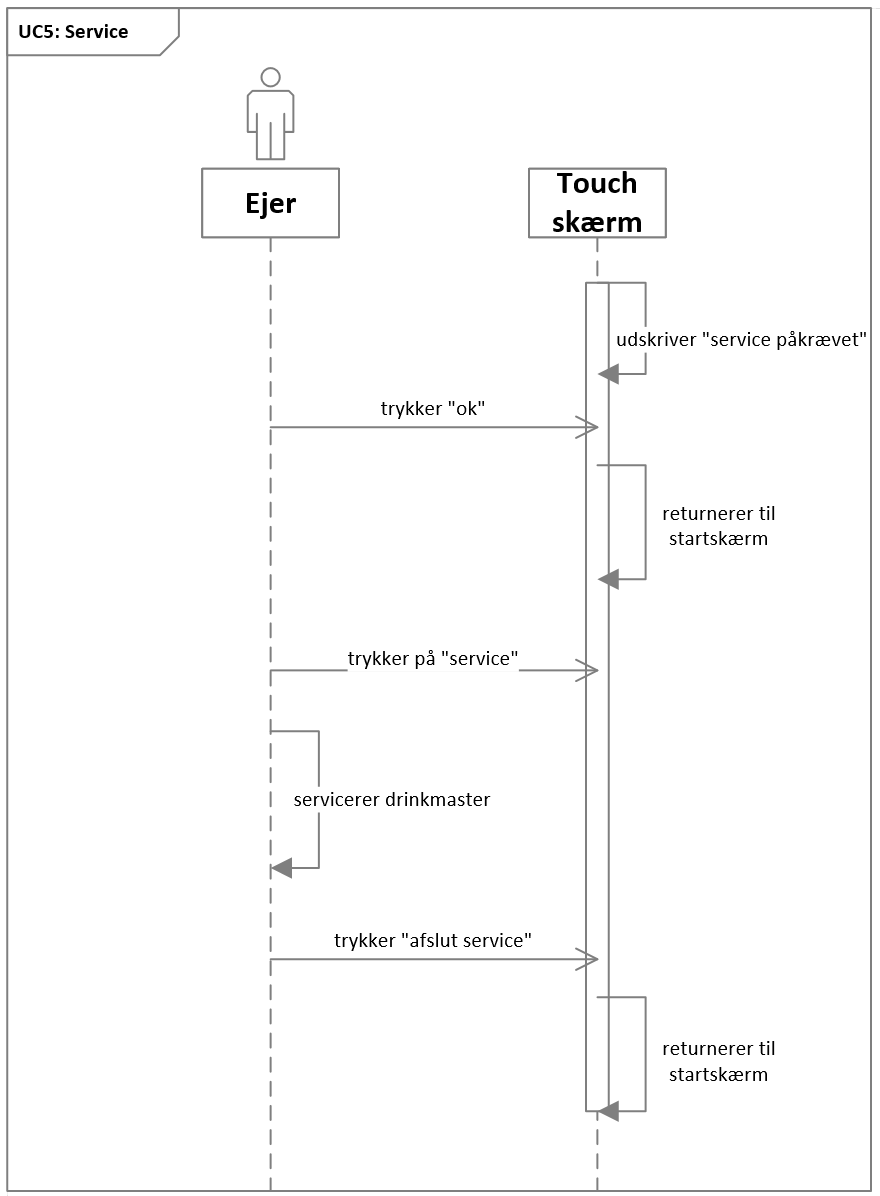
\includegraphics[width=1\textwidth]{Images/UC5service.png}
	\caption{Sekvensdiagram for UC5: Service}
	\label{fig:UC2_service}
\end{figure}

\subsection{Sekvensdiagrammer til test TUC'es}
%Test use case sekvensdiagrammer

\begin{figure}[H]
	\centering
	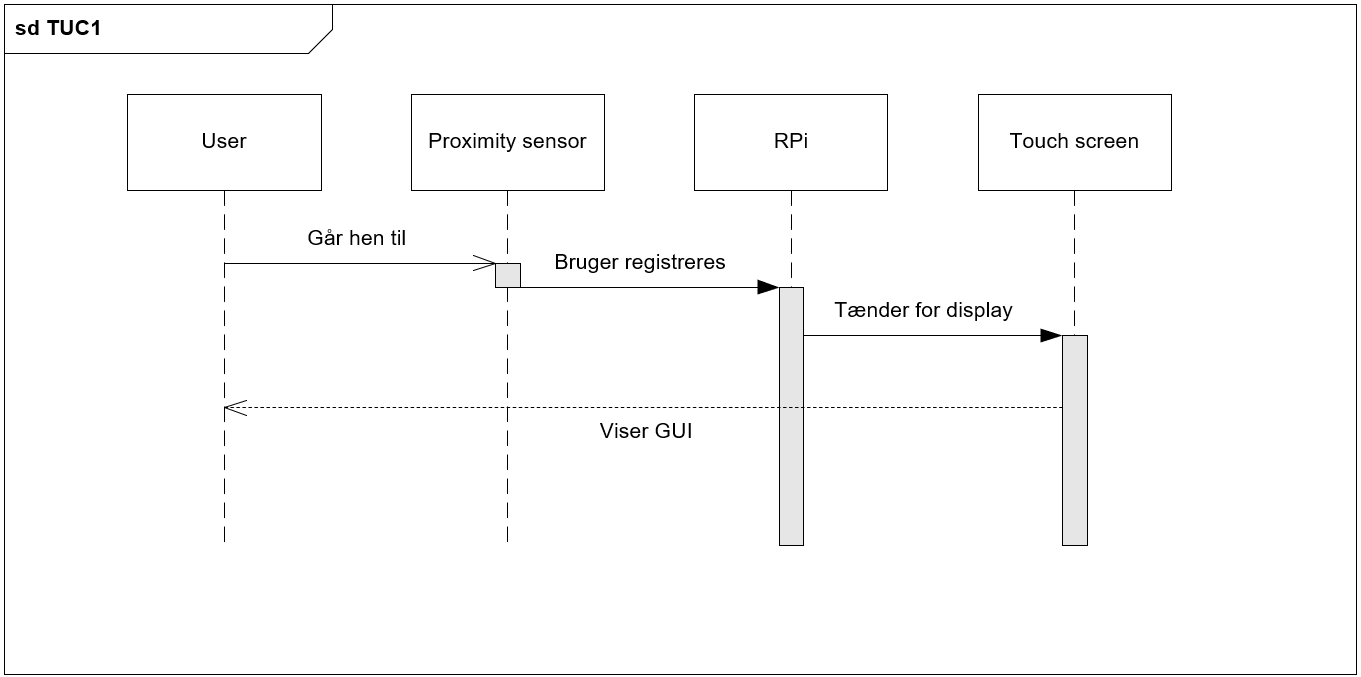
\includegraphics[width=1\textwidth]{Images/TUC1.png}
	\caption{Sekvensdiagram for test TUC1: Registrer bruger}
	\label{fig:testUC1}
\end{figure}

\begin{figure}[H]
	\centering
	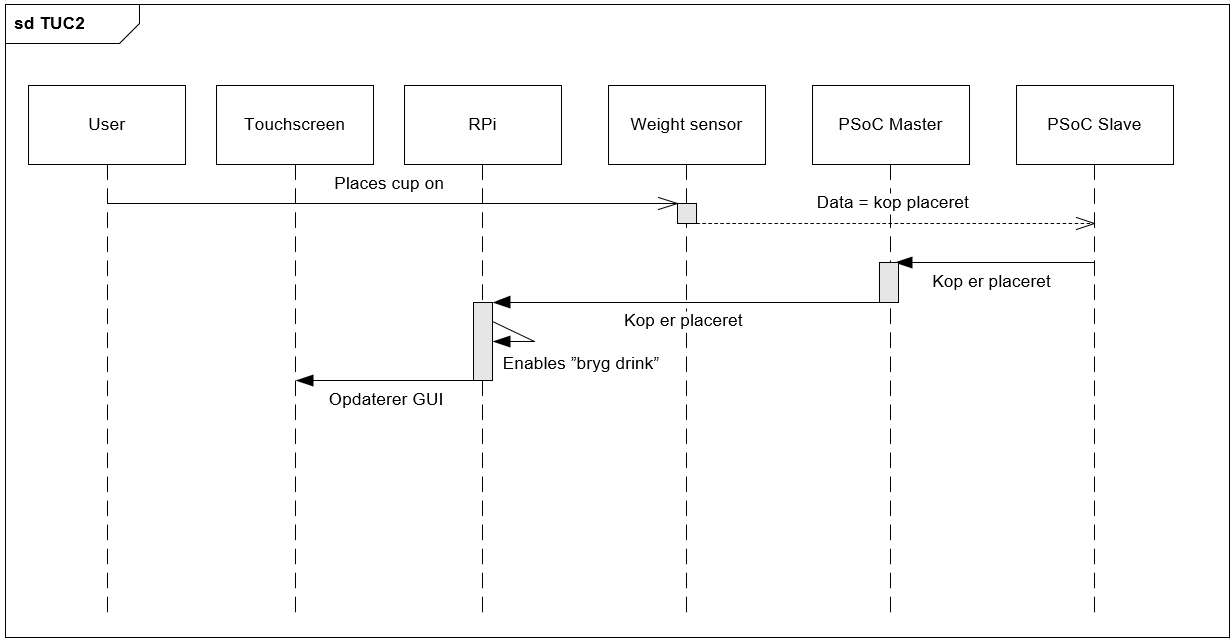
\includegraphics[width=1\textwidth]{Images/TUC2.png}
	\caption{Sekvensdiagram for test TUC2: Vægt registrerer kop}
	\label{fig:testUC2}
\end{figure}

\begin{figure}[H]
	\centering
	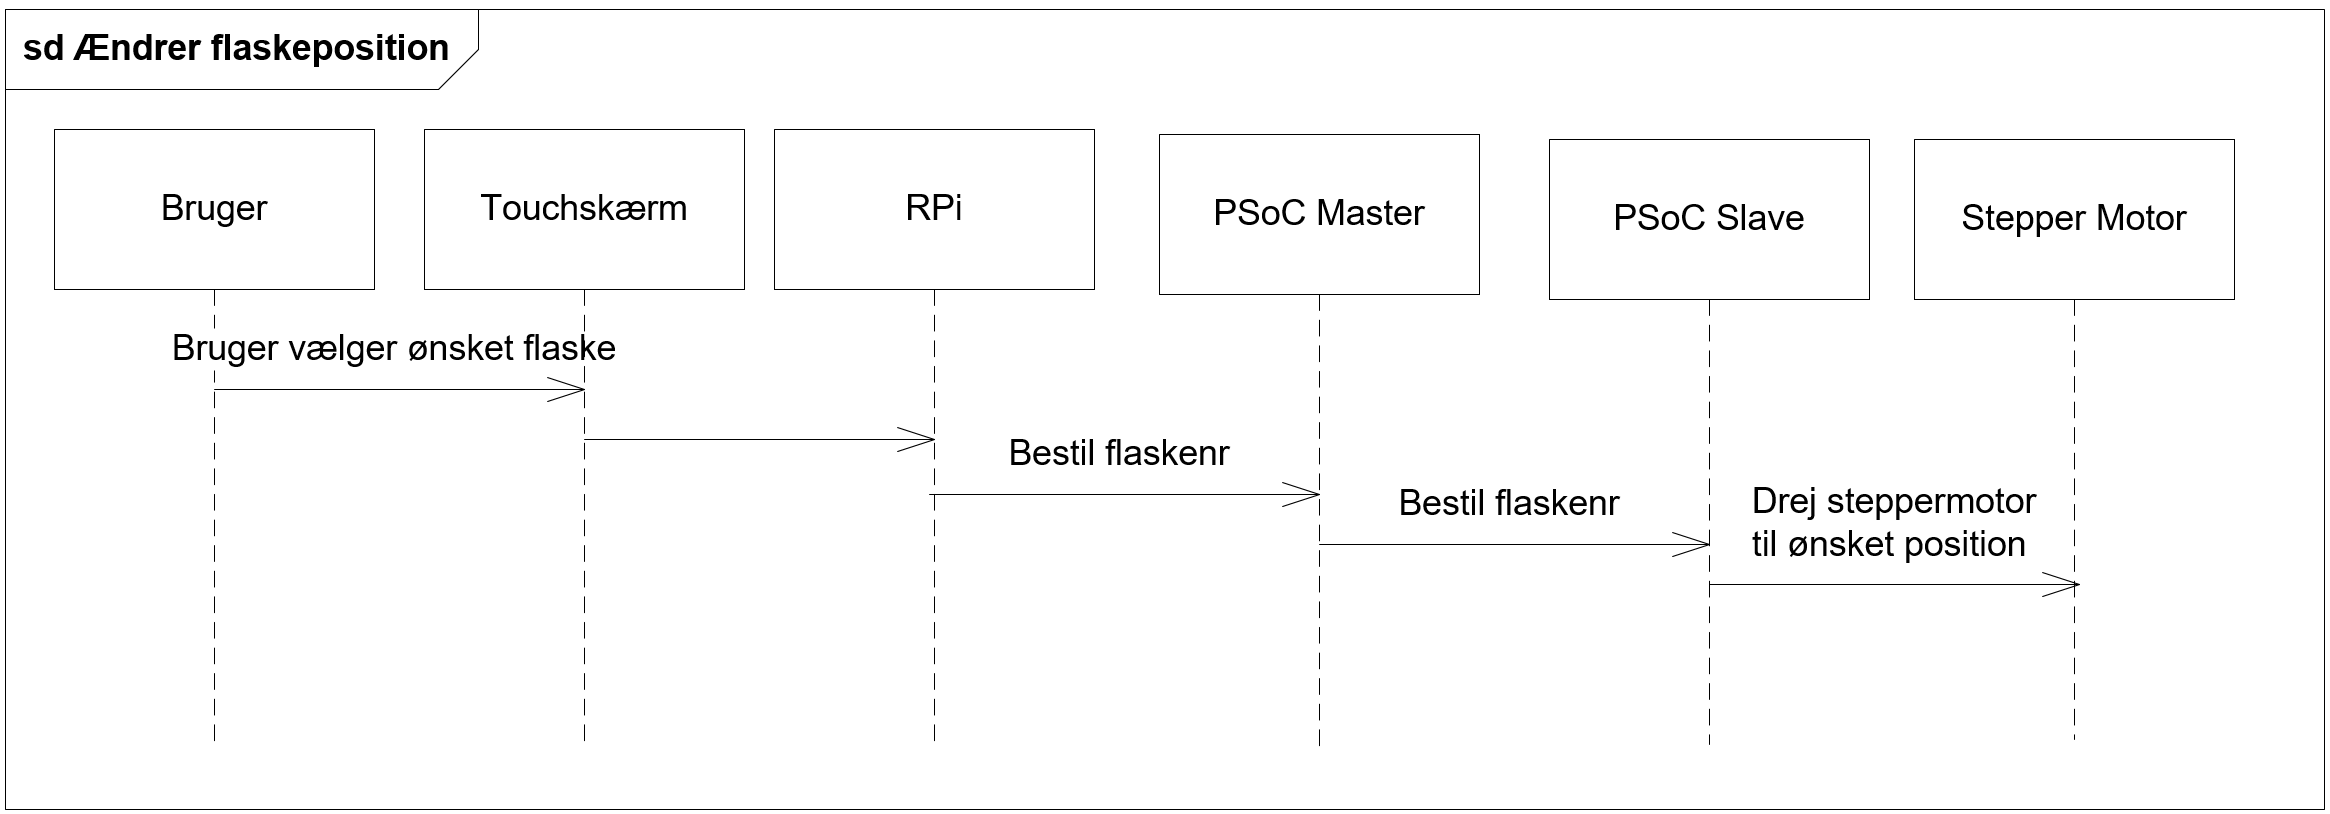
\includegraphics[width=1\textwidth]{Images/sdTestUC3.png}
	\caption{Sekvensdiagram for test TUC3: Ændrer flaskeposition}
	\label{fig:testUC3}
\end{figure}

\begin{figure}[H]
	\centering
	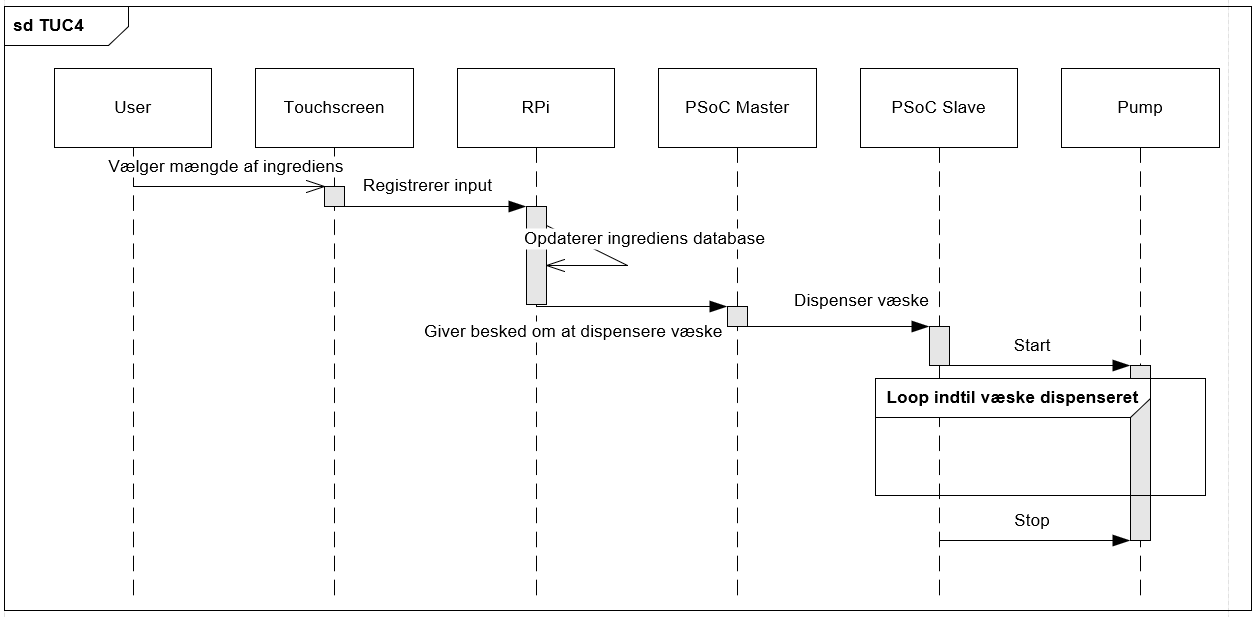
\includegraphics[width=1\textwidth]{Images/TUC4.png}
	\caption{Sekvensdiagram for test TUC4: Doser væske}
	\label{fig:testUC4}
\end{figure}
\begin{figure}[H]
	\centering
	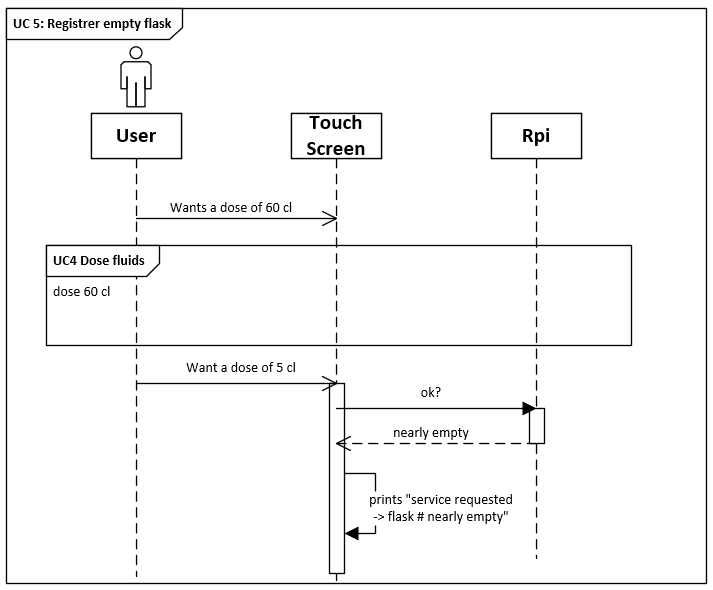
\includegraphics[width=1\textwidth]{Images/testUC5.png}
	\caption{Sekvensdiagram for test TUC5: Registrer tom flaske}
	\label{fig:testUC5}
\end{figure}

\begin{figure}[H]
    \centering
    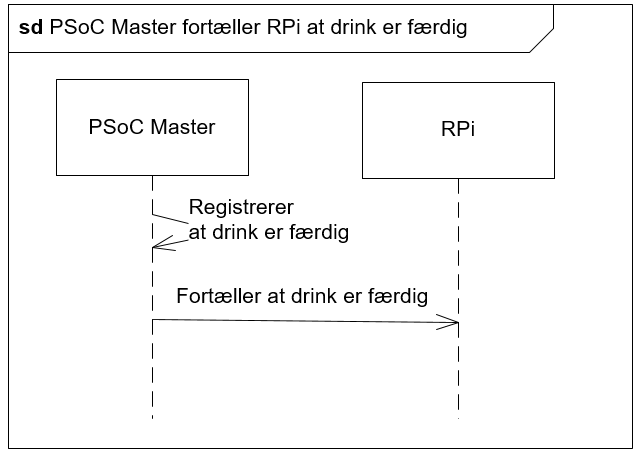
\includegraphics[width=1\textwidth]{Images/sdTestUC6.png}
    \caption{Sekvensdiagram for TUC6: PSoC Master fortæller RPi at drink er færdig}
    \label{fig:testUC6}
\end{figure}
\section{Applikationsmodeller}

\subsection{Applikationsmodel for RPi}
\subsubsection{UC1}

\begin{figure}[H]
    \centering
    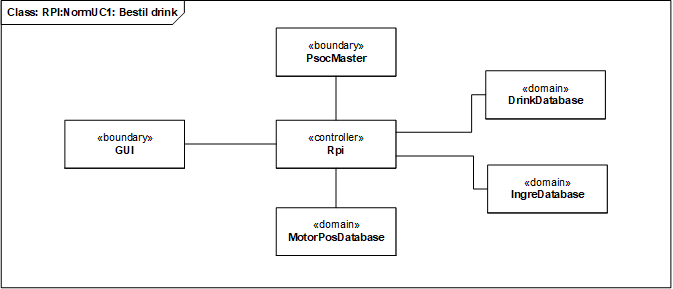
\includegraphics[width=1\textwidth]{Images/Applikationsmodeller/rpi/rpi_klassediagramNormUC1.png}
    \caption{Indledende klassediagram for Rpi i UC1}
    \label{fig:cdUC1Rpi}
\end{figure}

\begin{figure}[H]
    \centering
    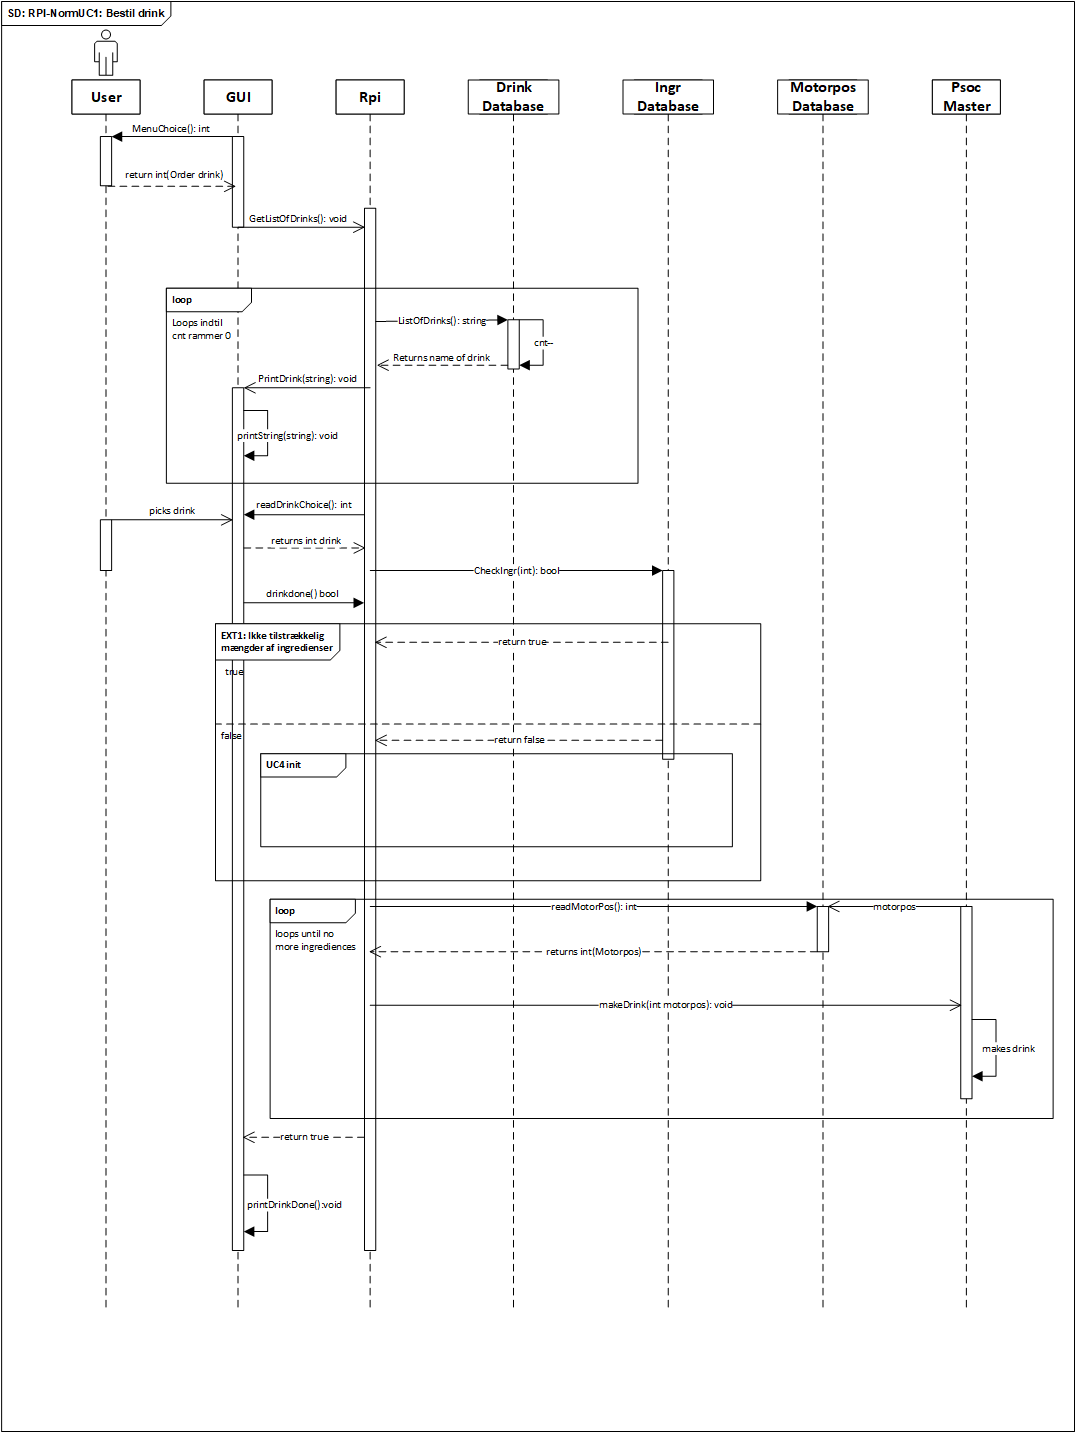
\includegraphics[width=1\textwidth]{Images/Applikationsmodeller/rpi/rpi_sekvensdiagramNormUC1.png}
    \caption{sekvensdiagram for Rpi i UC1}
    \label{fig:sdUC1Rpi}
\end{figure}

\begin{figure}[H]
    \centering
    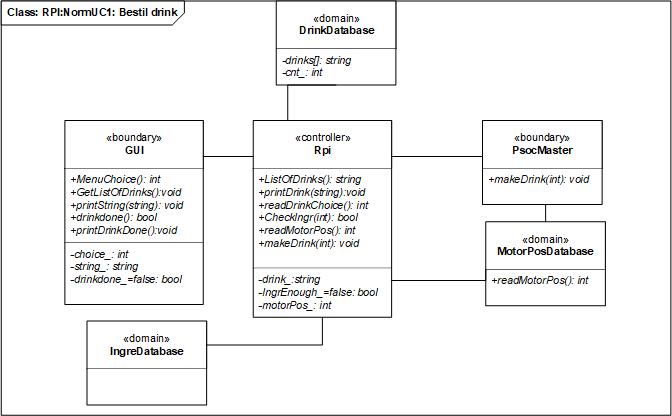
\includegraphics[width=1\textwidth]{Images/Applikationsmodeller/rpi/rpi_UdvidetklassediagramNormUC1.png}
    \caption{Udvidet klassediagram for Rpi i UC1}
    \label{fig:UcdUC1Rpi}
\end{figure}

\subsubsection{UC2}

\begin{figure}[H]
    \centering
    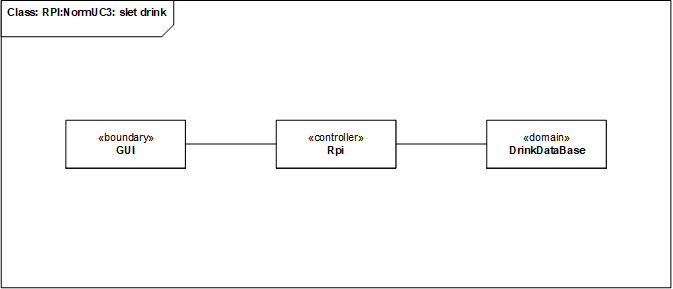
\includegraphics[width=1\textwidth]{Images/Applikationsmodeller/rpi/rpi_klassediagramNormUC3.png}
    \caption{Indledende klassediagram for Rpi i UC2}
    \label{fig:cdUC2Rpi}
\end{figure}

\begin{figure}[H]
    \centering
    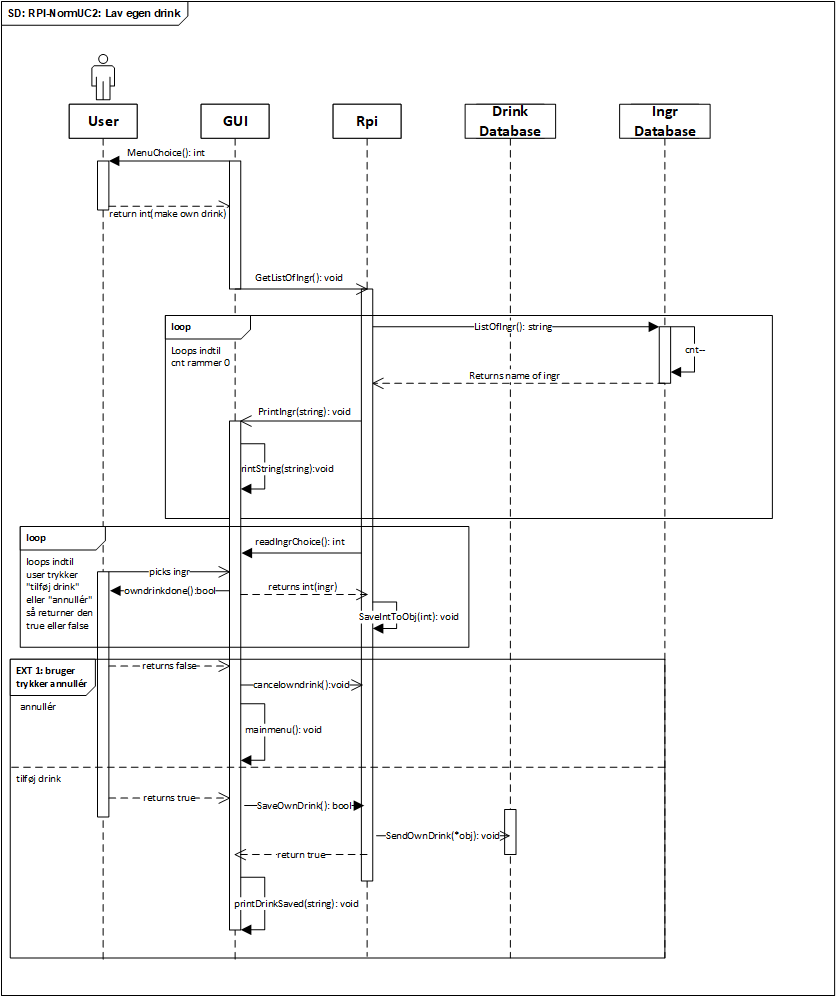
\includegraphics[width=1\textwidth]{Images/Applikationsmodeller/rpi/rpi_sekvensdiagramNormUC2.png}
    \caption{Sekvensdiagram for Rpi i UC2}
    \label{fig:sdUC2Rpi}
\end{figure}

\begin{figure}[H]
    \centering
    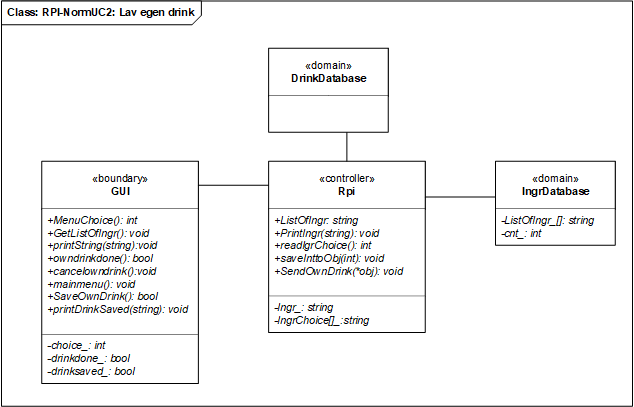
\includegraphics[width=1\textwidth]{Images/Applikationsmodeller/rpi/rpi_UdvidetklassediagramNormUC2.png}
    \caption{Udvidet klassediagram for Rpi i UC2}
    \label{fig:UcdUC2Rpi}
\end{figure}

\subsubsection{UC3}

\begin{figure}[H]
    \centering
    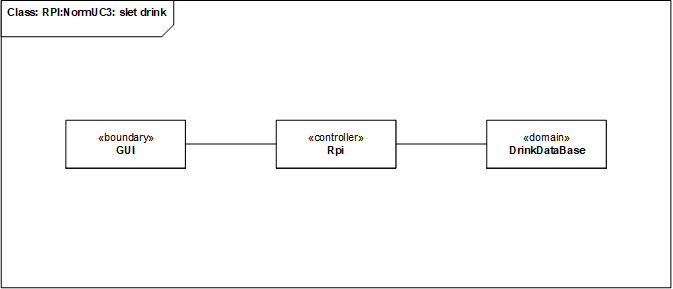
\includegraphics[width=1\textwidth]{Images/Applikationsmodeller/rpi/rpi_klassediagramNormUC3.png}
    \caption{Indledende klassediagram for Rpi i UC3}
    \label{fig:cdUC3Rpi}
\end{figure}

\begin{figure}[H]
    \centering
    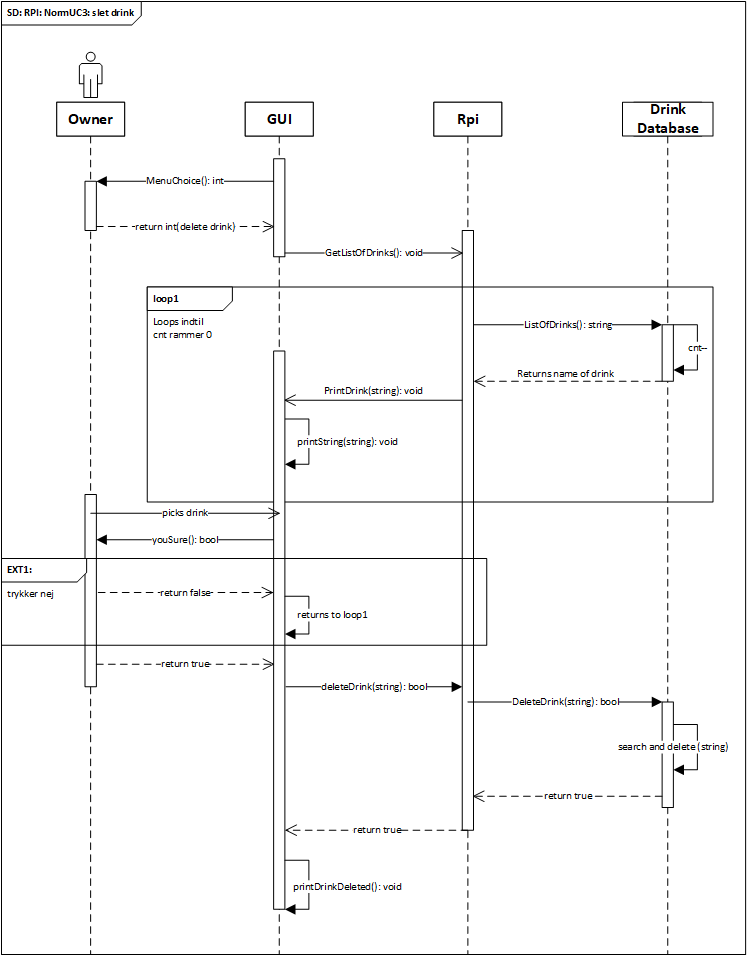
\includegraphics[width=1\textwidth]{Images/Applikationsmodeller/rpi/rpi_sekvensdiagramNormUC3.png}
    \caption{Sekvensdiagram for Rpi i UC3}
    \label{fig:SdUC3Rpi}
\end{figure}

\begin{figure}[H]
    \centering
    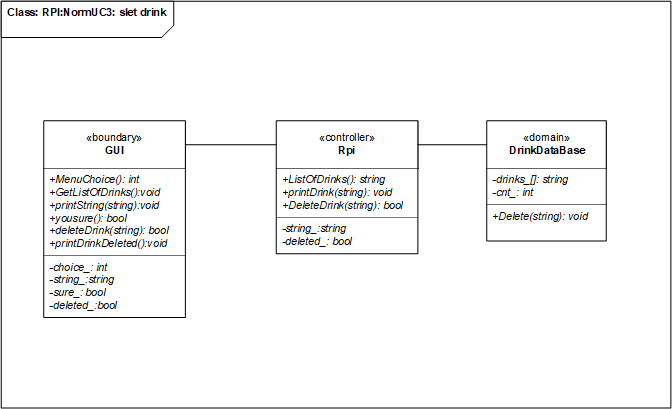
\includegraphics[width=1\textwidth]{Images/Applikationsmodeller/rpi/rpi_UdvidetklassediagramNormUC3.png}
    \caption{Udvidet klassediagram for Rpi i UC3}
    \label{fig:UcdUC3Rpi}
\end{figure}

\subsubsection{UC4}

\begin{figure}[H]
    \centering
    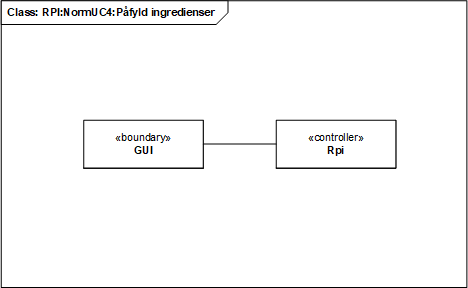
\includegraphics[width=1\textwidth]{Images/Applikationsmodeller/rpi/rpi_klassediagramNormUC4.png}
    \caption{Indledende klassediagram for Rpi i UC4}
    \label{fig:cdUC4Rpi}
\end{figure}

\begin{figure}[H]
    \centering
    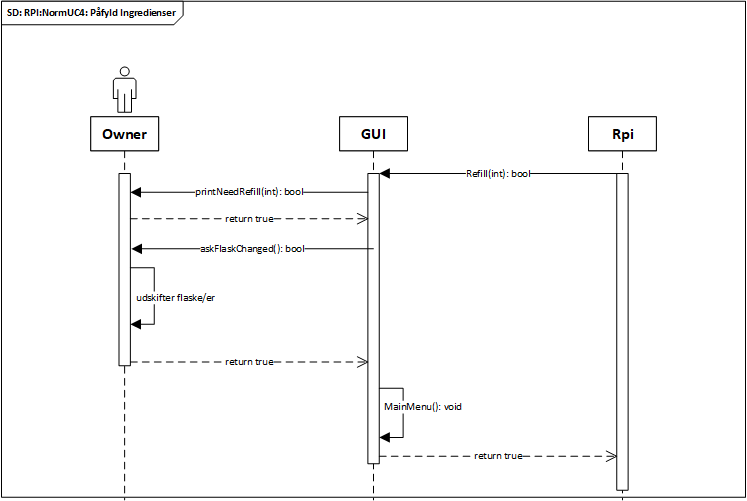
\includegraphics[width=1\textwidth]{Images/Applikationsmodeller/rpi/rpi_sekvensdiagramNormUC4.png}
    \caption{Sekvensdiagram for Rpi i UC4}
    \label{fig:sdUC4Rpi}
\end{figure}

\begin{figure}[H]
    \centering
    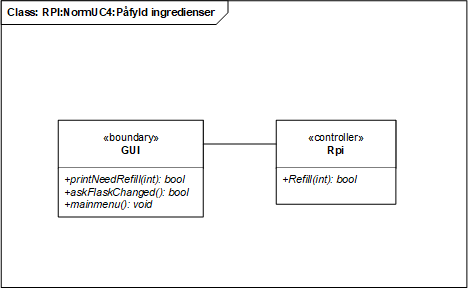
\includegraphics[width=1\textwidth]{Images/Applikationsmodeller/rpi/rpi_UdvidetklassediagramNormUC4.png}
    \caption{Udvidet klassediagram for Rpi i UC4}
    \label{fig:UcdUC4Rpi}
\end{figure}

\subsubsection{UC5}

\begin{figure}[H]
    \centering
    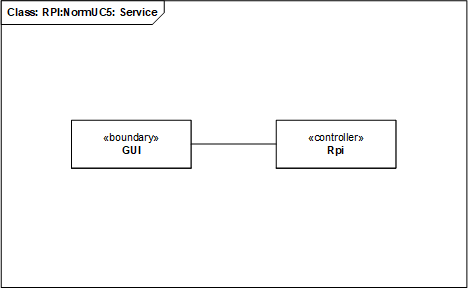
\includegraphics[width=1\textwidth]{Images/Applikationsmodeller/rpi/rpi_klassediagramNormUC5.png}
    \caption{Indledende klassediagram for Rpi i UC5}
    \label{fig:cdUC5Rpi}
\end{figure}

\begin{figure}[H]
    \centering
    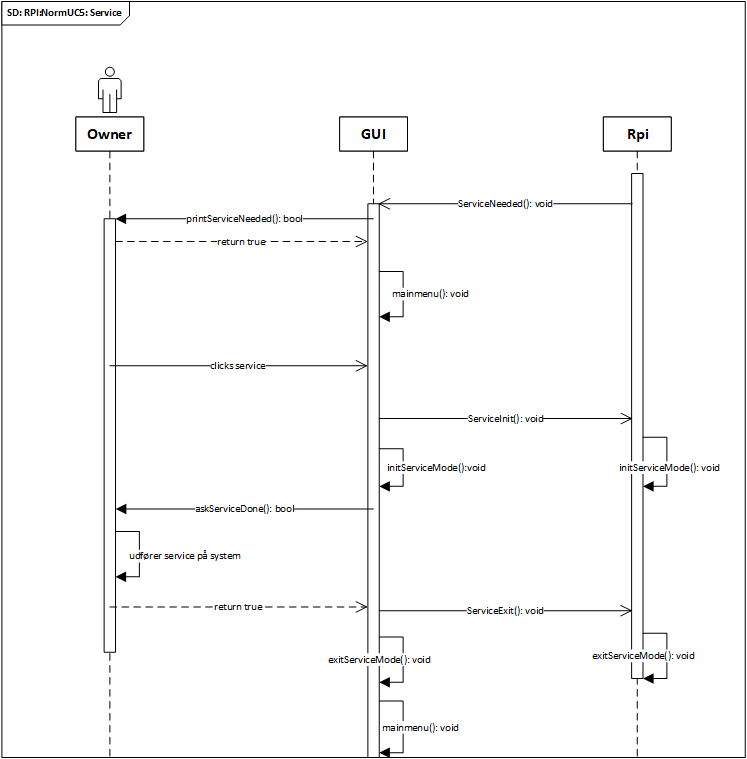
\includegraphics[width=1\textwidth]{Images/Applikationsmodeller/rpi/rpi_sekvensdiagramNormUC5.png}
    \caption{Sekvensdiagram for Rpi i UC5}
    \label{fig:sdUC4Rpi}
\end{figure}

\begin{figure}[H]
    \centering
    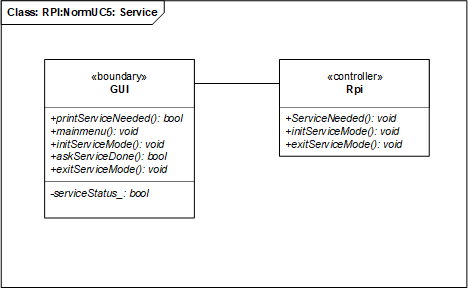
\includegraphics[width=1\textwidth]{Images/Applikationsmodeller/rpi/rpi_UdvidetklassediagramNormUC5.png}
    \caption{Udvidet klassediagram for Rpi i UC5}
    \label{fig:UcdUC5Rpi}
\end{figure}

\subsubsection{TUC1}

\begin{figure}[H]
    \centering
    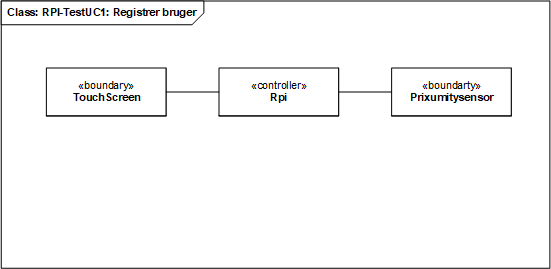
\includegraphics[width=1\textwidth]{Images/Applikationsmodeller/rpi/rpi_klassediagramTestUC1.png}
    \caption{Indledende klassediagram for Rpi i TUC1}
    \label{fig:cdTUC1Rpi}
\end{figure}

\begin{figure}[H]
    \centering
    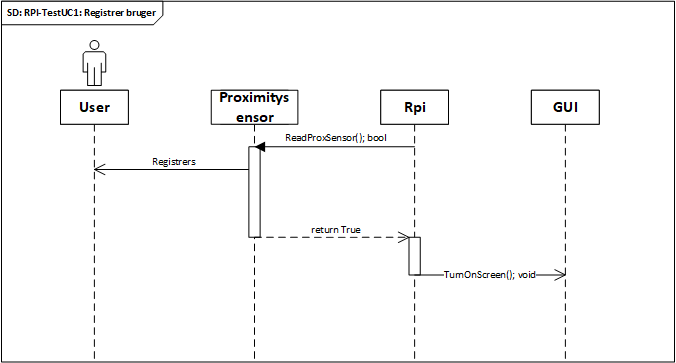
\includegraphics[width=1\textwidth]{Images/Applikationsmodeller/rpi/rpi_sekvensdiagramTestUC1.png}
    \caption{Sekvensdiagram for Rpi i TUC1}
    \label{fig:sdTUC1Rpi}
\end{figure}

\begin{figure}[H]
    \centering
    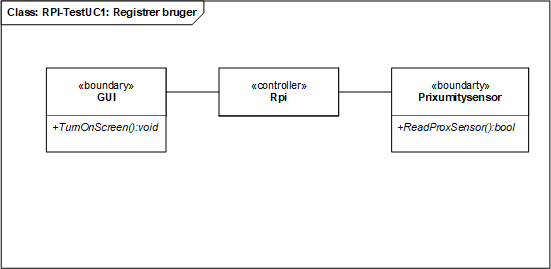
\includegraphics[width=1\textwidth]{Images/Applikationsmodeller/rpi/rpi_UdvidetklassediagramTestUC1.png}
    \caption{Udvidet klassediagram for Rpi i TUC1}
    \label{fig:UcdTUC1Rpi}
\end{figure}

\subsubsection{TUC2}

\begin{figure}[H]
    \centering
    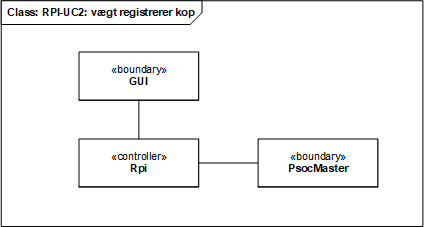
\includegraphics[width=1\textwidth]{Images/Applikationsmodeller/rpi/rpi_klassediagramTestUC2.png}
    \caption{Indledende klassediagram for Rpi i TUC2}
    \label{fig:cdTUC2Rpi}
\end{figure}

\begin{figure}[H]
    \centering
    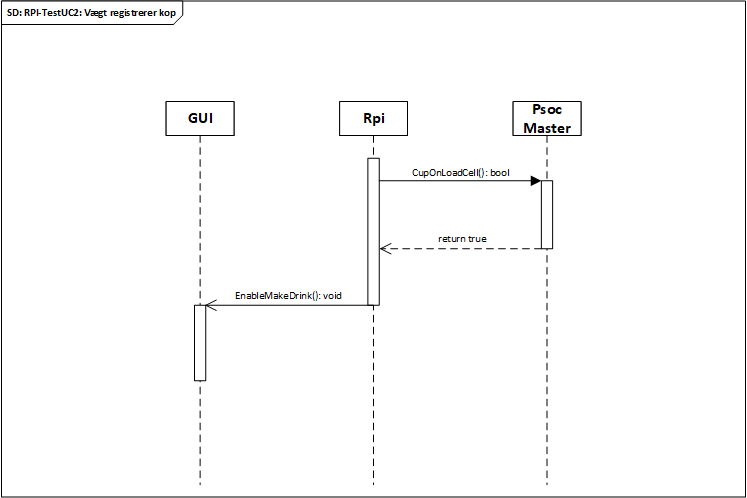
\includegraphics[width=1\textwidth]{Images/Applikationsmodeller/rpi/rpi_sekvensdiagramTestUC2.png}
    \caption{Sekvensdiagram for Rpi i TUC2}
    \label{fig:sdTUC2Rpi}
\end{figure}

\begin{figure}[H]
    \centering
    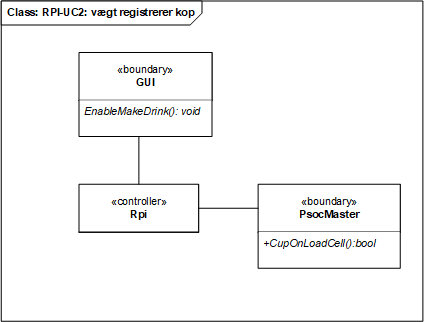
\includegraphics[width=1\textwidth]{Images/Applikationsmodeller/rpi/rpi_UdvidetklassediagramTestUC2.png}
    \caption{Udvidet klassediagram for Rpi i TUC2}
    \label{fig:UcdTUC2Rpi}
\end{figure}

\subsubsection{TUC3}

\begin{figure}[H]
    \centering
    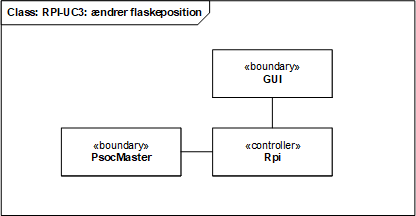
\includegraphics[width=1\textwidth]{Images/Applikationsmodeller/rpi/rpi_klassediagramTestUC3.png}
    \caption{Indledende klassediagram for Rpi i TUC3}
    \label{fig:cdTUC3Rpi}
\end{figure}

\begin{figure}[H]
    \centering
    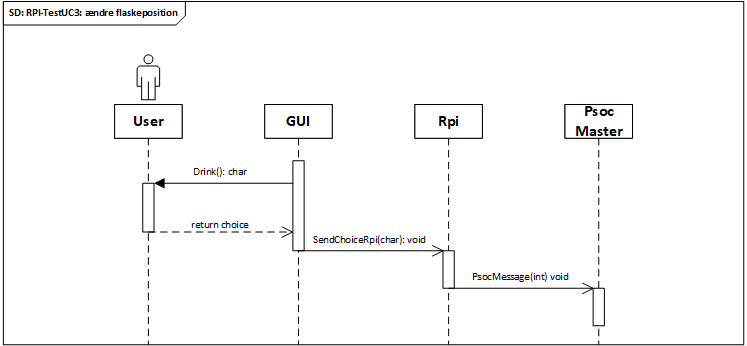
\includegraphics[width=1\textwidth]{Images/Applikationsmodeller/rpi/rpi_sekvensdiagramTestUC3.png}
    \caption{Sekvensdiagram for Rpi i TUC3}
    \label{fig:sdTUC3Rpi}
\end{figure}

\begin{figure}[H]
    \centering
    \includegraphics[width=1\textwidth]{Images/Applikationsmodeller/rpi/rpi_UdvidetklassediagramTestUC3.png}
    \caption{Udvidet klassediagram for Rpi i TUC3}
    \label{fig:UcdTUC3Rpi}
\end{figure}

\subsubsection{TUC4}

\begin{figure}[H]
    \centering
    \includegraphics[width=1\textwidth]{Images/Applikationsmodeller/rpi/rpi_klassediagramTestUC4.png}
    \caption{Indledende klassediagram for Rpi i TUC4}
    \label{fig:cdTUC4Rpi}
\end{figure}

\begin{figure}[H]
    \centering
    \includegraphics[width=1\textwidth]{Images/PsocSlaveTUC4.jpg}
    \caption{Indledende klassediagram for Psoc slave i TUC4}
    \label{fig:cdTUC4Rpi}
\end{figure}


\begin{figure}[H]
    \centering
    \includegraphics[width=1\textwidth]{Images/Applikationsmodeller/rpi/rpi_sekvensdiagramTestUC4.png}
    \caption{Sekvensdiagram for Rpi i TUC4}
    \label{fig:sdTUC4Rpi}
\end{figure}

\begin{figure}[H]
    \centering
    \includegraphics[width=1\textwidth]{Images/Applikationsmodeller/rpi/rpi_UdvidetklassediagramTestUC4.png}
    \caption{Udvidet klassediagram for Rpi i TUC4}
    \label{fig:UcdTUC4Rpi}
\end{figure}

\subsubsection{TUC5}

\begin{figure}[H]
    \centering
    \includegraphics[width=1\textwidth]{Images/Applikationsmodeller/rpi/rpi_klassediagramTestUC5.png}
    \caption{Indledende klassediagram for Rpi i TUC5}
    \label{fig:cdTUC5Rpi}
\end{figure}

\begin{figure}[H]
    \centering
    \includegraphics[width=1\textwidth]{Images/Applikationsmodeller/rpi/rpi_sekvensdiagramTestUC5.png}
    \caption{Sekvensdiagram for Rpi i TUC5}
    \label{fig:sdTUC5Rpi}
\end{figure}

\begin{figure}[H]
    \centering
    \includegraphics[width=1\textwidth]{Images/Applikationsmodeller/rpi/rpi_UdvidetklassediagramTestUC5.png}
    \caption{Udvidet klassediagram for Rpi i TUC5}
    \label{fig:UcdTUC5Rpi}
\end{figure}

\subsubsection{TUC6}

\begin{figure}[H]
    \centering
    \includegraphics[width=1\textwidth]{Images/Applikationsmodeller/rpi/rpi_klassediagramTestUC6.png}
    \caption{Indledende klassediagram for Rpi i TUC6}
    \label{fig:cdTUC6Rpi}
\end{figure}

\begin{figure}[H]
    \centering
    \includegraphics[width=1\textwidth]{Images/Applikationsmodeller/rpi/rpi_sekvensdiagramTestUC6.png}
    \caption{Sekvensdiagram for Rpi i TUC6}
    \label{fig:sdTUC6Rpi}
\end{figure}

\begin{figure}[H]
    \centering
    \includegraphics[width=1\textwidth]{Images/Applikationsmodeller/rpi/rpi_UdvidetklassediagramTestUC6.png}
    \caption{Udvidet klassediagram for Rpi i TUC6}
    \label{fig:UcdTUC6Rpi}
\end{figure}

\subsubsection{Samlet klassediagram for Rpi}

\begin{figure}[H]
    \centering
    \includegraphics[width=1\textwidth]{Images/Applikationsmodeller/rpi/Samlet_klassediagram.png}
    \caption{Samlet klassediagram for Rpi}
    \label{fig:Samlet - Rpi}
\end{figure}

\subsection{Applikationsmodel for PSoC Master}
\subsubsection{UC1}

\begin{figure}[H]
	\centering
	\includegraphics[width=1\textwidth]{Images/Applikationsmodeller/PSoCMaster/UC1_cd_PSoC_Master.png}
	\caption{Indledende klassediagram for PSoC Master UC1}
	\label{fig:cdUC1PSoCMaster}
\end{figure}

\begin{figure}[H]
	\centering
	\includegraphics[width=1\textwidth]{Images/Applikationsmodeller/PSoCMaster/UC1_sd_PSoC_Master.png}
	\caption{Sekvensdiagram for UC1 PSoC Master}
	\label{fig:sdUC1PSoCMaster}
\end{figure}

\begin{figure}[H]
	\centering
	\includegraphics[width=1\textwidth]{Images/Applikationsmodeller/PSoCMaster/UC1_cd_PSoC_Master_final.png}
	\caption{Færdigt klassediagram for UC1 PSoC Master}
	\label{fig:cdUC1PSoCMaster_final}
\end{figure}

\subsubsection{TUC2}

\begin{figure}[H]
	\centering
	\includegraphics[width=1\textwidth]{Images/Applikationsmodeller/PSoCMaster/TUC2_cd_PSoC_Master.png}
	\caption{Klassediagram for TUC2 PSoC Master}
	\label{fig:cdTUC2PSoCMaster}
\end{figure}

\begin{figure}[H]
	\centering
	\includegraphics[width=1\textwidth]{Images/Applikationsmodeller/PSoCMaster/TUC2_sd_PSoC_Master.png}
	\caption{Sekvendiagram for TUC2 PSoC Master}
	\label{fig:sdTUC2PSoCMaster}
\end{figure}

\begin{figure}[H]
	\centering
	\includegraphics[width=1\textwidth]{Images/Applikationsmodeller/PSoCMaster/TUC2_cd_PSoC_Master_final.png}
	\caption{Færdigt klassediagram for TUC2 PSoC Master}
	\label{fig:cdTUC2PSoCMaster_final}
\end{figure}

\subsubsection{TUC3}
\begin{figure}[H]
	\centering
	\includegraphics[width=1\textwidth]{Images/Applikationsmodeller/PSoCMaster/TUC3_cd_PSoC_Master.png}
	\caption{Klassediagram for TUC3 PSoC Master}
	\label{fig:cdTUC3PSoCMaster}
\end{figure}

\begin{figure}[H]
	\centering
	\includegraphics[width=1\textwidth]{Images/Applikationsmodeller/PSoCMaster/TUC3_sd_PSoC_Master.png}
	\caption{Sekvensdiagram for TUC3 PSoC Master}
	\label{fig:sdTUC3PSoCMaster}
\end{figure}

\begin{figure}[H]
	\centering
	\includegraphics[width=1\textwidth]{Images/Applikationsmodeller/PSoCMaster/TUC3_cd_PSoC_Master_final.png}
	\caption{Færdigt klassediagram for TUC3 PSoC Master}
	\label{fig:cdTUC3PSoCMaster_final}
\end{figure}
\subsubsection{TUC4}
\begin{figure}[H]
	\centering
	\includegraphics[width=1\textwidth]{Images/Applikationsmodeller/PSoCMaster/TUC4_cd_PSoC_Master.png}
	\caption{Klassediagram for TUC4 PSoC Master}
	\label{fig:cdTUC4PSoCMaster}
\end{figure}

\begin{figure}[H]
	\centering
	\includegraphics[width=1\textwidth]{Images/Applikationsmodeller/PSoCMaster/TUC4_sd_PSoC_Master.png}
	\caption{Sekvensdiagram for TUC4 PSoC Master}
	\label{fig:sdTUC3PSoCMaster}
\end{figure}
\begin{figure}[H]
	\centering
	\includegraphics[width=1\textwidth]{Images/Applikationsmodeller/PSoCMaster/TUC4_cd_PSoC_Master_final.png}
	\caption{Færdigt klassediagram for TUC4 PSoC Master}
	\label{fig:cdTUC4PSoCMaster_final}
\end{figure}

\subsubsection{TUC6 - PSoC Master fortæller RPi at drink er færdig}
\begin{figure}[H]
	\centering
	\includegraphics[width=1\textwidth]{Images/Applikationsmodeller/PSoCMaster/class1.png}
	\caption{Første klassediagram for TUC6 for PSoC Master}
	\label{fig:cdTUC6PSoCMaster_first}
\end{figure}

\begin{figure}[H]
	\centering
	\includegraphics[width=1\textwidth]{Images/Applikationsmodeller/PSoCMaster/PSoCMasterTUC6_Sekvensdiagram.png}
	\caption{Sekvensdiagram for TUC6 PSoC Master}
	\label{fig:sdTUC6PSoCMaster}
\end{figure}

\begin{figure}[H]
	\centering
	\includegraphics[width=1\textwidth]{Images/Applikationsmodeller/PSoCMaster/PSoCMasterTUC6_Udv_class.png}
	\caption{Færdigt klassediagram for TUC6 -  PSoC Master}
	\label{fig:cdTUC6PSoCMaster_final}
\end{figure}

\subsection{Applikationsmodel for PSoC Slaven - Vægtsensor}

\subsubsection{UC1}
\begin{figure}[H]
	\centering
	\includegraphics[width=1\textwidth]{Images/Applikationsmodeller/PSoCWeight/classAppWeightUC1.png}
	\caption{Klassediagram for "PSoC slave weight" UC1}
	\label{fig:classAppWeightUC1}
\end{figure}

\begin{figure}[H]
	\centering
	\includegraphics[width=1\textwidth]{Images/Applikationsmodeller/PSoCWeight/sdAppWeightUC1.png}
	\caption{Sekvensdiagram for "PSoC slave weight" UC1}
	\label{fig:sdAppWeightUC1}
\end{figure}

\begin{figure}[H]
	\centering
	\includegraphics[width=1\textwidth]{Images/Applikationsmodeller/PSoCWeight/ClassExtAppWeightUC1.png}
	\caption{Udvidet klassediagram for "PSoC slave weight" UC1}
	\label{fig:ClassExtAppWeightUC1}
\end{figure}

\subsubsection{TUC2}
\begin{figure}[H]
	\centering
	\includegraphics[width=1\textwidth]{Images/Applikationsmodeller/PSoCWeight/Class_TUC2_PSoC_Slave_Weight.png}
	\caption{Klassediagram for "PSoC slave weight" TUC2}
	\label{fig:cdTUC2PSoCSlaveWeight}
\end{figure}

%\subsubsection{TUC2}
\begin{figure}[H]
	\centering
	\includegraphics[width=1\textwidth]{Images/Applikationsmodeller/PSoCWeight/Sd_TUC2_PSoC_Slave_Weight_Temporary_Crop.png}
	\caption{Sekvensdiagram "PSoC slave weight" TUC2}
	\label{fig:sdTUC2PSoCSlaveWeight}
\end{figure}

%\subsubsection{TUC2}
\begin{figure}[H]
	\centering
	\includegraphics[width=1\textwidth]{Images/Applikationsmodeller/PSoCWeight/Class_TUC2_PSoC_Slave_Weight.png}
	\caption{Klassediagram for "PSoC slave weight" TUC2}
	\label{fig:classTUC2PSoCSlaveWeight}
\end{figure}

\subsection{Applikationsmodel for PSoC Slaven - Pumpestyring}
\subsubsection{UC1}
\begin{figure}[H]
	\centering
	\includegraphics[width=1\textwidth]{Images/Applikationsmodeller/UC1_cd_PSoC_Slave_pump.png}
	\caption{Klassediagram for "PSoC slave pump" UC1}
	\label{fig:cdUC1PSoCSlavePump}
\end{figure}

\begin{figure}[H]
	\centering
	\includegraphics[width=1\textwidth]{Images/Applikationsmodeller/UC1_sd_PSoC_Slave_pump.png}
	\caption{Sekvensdiagram for PSoC Slave Pump UC1}
	\label{fig:sdUC1PSoCSlavePump}
\end{figure}

\begin{figure}[H]
	\centering
	\includegraphics[width=1\textwidth]{Images/Applikationsmodeller/UC1_cd_PSoC_Slave_pump_final.png}
	\caption{Færdigt klassediagram for UC1 PSoC Slave Pump}
	\label{fig:cdUC1PSoCSlavePump_final}
\end{figure}


\subsection{Applikationsmodel for PSoC Slaven - Steppermotor}
\subsubsection{UC1}
\begin{figure}[H]
	\centering
	\includegraphics[width=1\textwidth]{Images/Applikationsmodeller/PSoCStepper/ClassSteppermotorUC1.png}
	\caption{Indledende klassediagram for PSoC Slave - Steppermotor UC1}
	\label{fig:preClassStepperUC1}
\end{figure}

\begin{figure}[H]
	\centering
	\includegraphics[width=1\textwidth]{Images/Applikationsmodeller/PSoCStepper/sdSteppermotorUC1.png}
	\caption{Sekvensdiagram for PSoC Slave - Steppermotor UC1}
	\label{fig:sdStepperUC1}
\end{figure}

\begin{figure}[H]
	\centering
	\includegraphics[width=1\textwidth]{Images/Applikationsmodeller/PSoCStepper/ClassextSteppermotorUC1.png}
	\caption{Udvidet klassediagram for PSoC Slave - Steppermotor UC1}
	\label{fig:postClassStepperUC1}
\end{figure}

\subsubsection{TUC3}
\begin{figure}[H]
	\centering
	\includegraphics[width=1\textwidth]{Images/Applikationsmodeller/PSoCStepper/first_class_TUC_3_PSoC_Slave_steppermotor.png}
	\caption{Klassediagram for PSoC Slave - Steppermotor TUC3}
	\label{fig:preClassStepperTUC3}
\end{figure}

\begin{figure}[H]
	\centering
	\includegraphics[width=1\textwidth]{Images/Applikationsmodeller/PSoCStepper/sd_TUC_3_PSoC_Slave_steppermotor.png}
	\caption{Sekvensdiagram for PSoC Slave - Steppermotor TUC3}
	\label{fig:sdStepperTUC3}
\end{figure}

\begin{figure}[H]
	\centering
	\includegraphics[width=1\textwidth]{Images/Applikationsmodeller/PSoCStepper/second_class_TUC_3_PSoC_Slave_steppermotor.png}
	\caption{Udvidet klassediagram for PSoC Slave - Steppermotor TUC3}
	\label{fig:postClassStepperTUC3}
\end{figure}


\end{document}